\chapter{Additional Examples}\label{additional}

This chapter contains additional examples of DAKOTA methods and
verification test problems. While the test problems and binary
analysis drivers are principally managed in {\tt Dakota/test}, many
extracted input files are also included in {\tt Dakota/examples/methods} 
for user convenience.

\section{Textbook Examples}\label{additional:textbook}

The two-variable version of the ``textbook'' test problem provides
a nonlinearly constrained optimization test case. It is formulated as:
\begin{eqnarray}
\texttt{minimize }
& & f = (x_1-1)^{4}+(x_2-1)^{4}     \nonumber \\
\texttt{subject to }
& & g_1 = x_1^2-\frac{x_2}{2} \le 0 \nonumber \\
& & g_2 = x_2^2-\frac{x_1}{2} \le 0 \label{additional:textbook_f} \\
& &  0.5 \le x_1 \le 5.8            \nonumber \\
& & -2.9 \le x_2 \le 2.9            \nonumber
\end{eqnarray}

Contours of this example problem are illustrated in
Figure~\ref{additional:textbook_prob}(a), with a close-up view of
the feasible region given in
Figure~\ref{additional:textbook_prob}(b).

\begin{figure}[htp!]
  \centering
  \begin{tabular}{cc}
  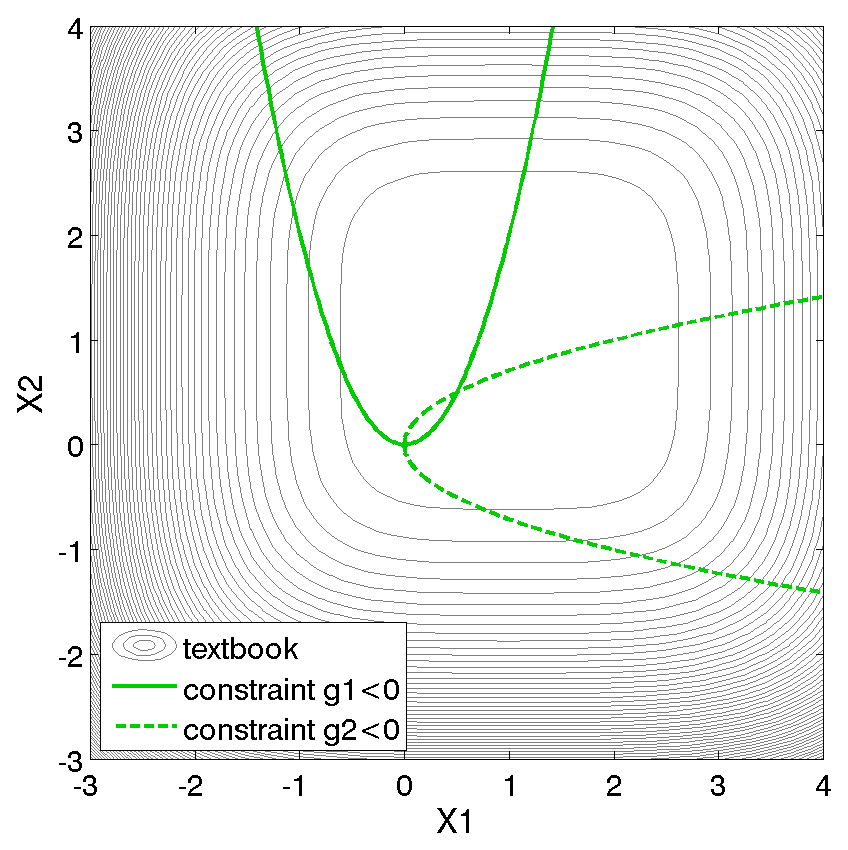
\includegraphics[height=2.5in]{images/textbook_contours} &
  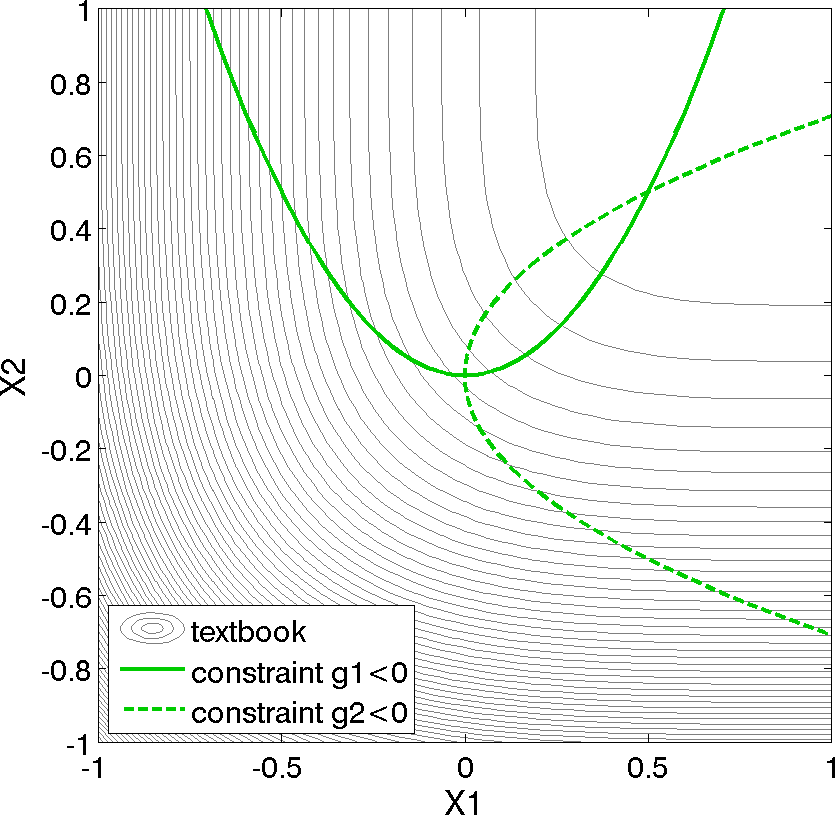
\includegraphics[height=2.5in]{images/textbook_closeup} \\
  (a) & (b) \\
  \end{tabular}
  \caption{Contours of the textbook problem (a) on the $[-3,4] \times
    [-3,4]$ domain and (b) zoomed into an area containing the
    constrained optimum point $(x_1,x_2) = (0.5,0.5)$. The
    feasible region lies at the intersection of the two constraints
    $g_1$ (solid) and $g_2$ (dashed).}
  \label{additional:textbook_prob}
\end{figure}

For the textbook test problem, the unconstrained minimum occurs at
$(x_1,x_2) = (1,1)$. However, the inclusion of the constraints
moves the minimum to $(x_1,x_2) = (0.5,0.5)$.
Equation~\ref{additional:textbook_f} presents the 2-dimensional
form of the textbook problem. An extended formulation is stated as
\begin{eqnarray}
\texttt{minimize }   & & f = \sum_{i=1}^{n}(x_i-1)^4 \nonumber\\
\texttt{subject to } & & g_1 = x_1^2-\frac{x_2}{2} \leq 0
  \label{additional:tbe}\\
  & & g_2=x_2^2-\frac{x_1}{2} \leq 0\nonumber\\
  & & 0.5 \leq x_1 \leq 5.8\nonumber\\
  & & -2.9 \leq x_2 \leq 2.9\nonumber
\end{eqnarray}
where $n$ is the number of design variables. The objective function is
designed to accommodate an arbitrary number of design variables in
order to allow flexible testing of a variety of data sets. Contour
plots for the $n=2$ case have been shown previously in
Figure~\ref{additional:textbook_prob}.

For the optimization problem given in Equation~\ref{additional:tbe}, the
unconstrained solution\\(\texttt{num\_nonlinear\_inequality\_constraints} 
set to zero) for two design variables is:
\begin{eqnarray*}
    x_1 &=& 1.0 \\
    x_2 &=& 1.0
\end{eqnarray*}
with
\begin{eqnarray*}
    f^{\ast} &=& 0.0
\end{eqnarray*}

The solution for the optimization problem constrained by $g_1$\\
(\texttt{num\_nonlinear\_inequality\_constraints} set to one) is:
\begin{eqnarray*}
    x_1 &=& 0.763 \\
    x_2 &=& 1.16
\end{eqnarray*}
with
\begin{eqnarray*}
      f^{\ast} &=& 0.00388 \\
    g_1^{\ast} &=& 0.0 ~~\mathrm{(active)}
\end{eqnarray*}

The solution for the optimization problem constrained by $g_1$ and $g_2$\\
(\texttt{num\_nonlinear\_inequality\_constraints} set to two) is:
\begin{eqnarray*}
    x_1 &=& 0.500 \\
    x_2 &=& 0.500
\end{eqnarray*}
with
\begin{eqnarray*}
      f^{\ast} &=& 0.125 \\
    g_1^{\ast} &=& 0.0 ~~\mathrm{(active)} \\
    g_2^{\ast} &=& 0.0 ~~\mathrm{(active)}
\end{eqnarray*}

Note that as constraints are added, the design freedom is restricted
(the additional constraints are active at the solution) and an
increase in the optimal objective function is observed.

\subsection{Examples}\label{additional:textbook:examples}

\subsubsection{Gradient-based Constrained Optimization}\label{additional:textbook:examples:gradient2}

This example demonstrates the use of a gradient-based optimization
algorithm on a nonlinearly constrained problem. The 
DAKOTA input file for this example problem is
shown in Figure~\ref{additional:textbook_grad_constr}. This
input file is similar to the input file for the unconstrained
gradient-based optimization example problem involving the Rosenbrock
function, seen in Section~\ref{tutorial:examples:optimization}. 
Note the addition of commands in the responses block of
the input file that identify the number and type of constraints, along
with the upper bounds on these constraints. The commands
\texttt{direct} and \texttt{analysis\_driver = 'text\_book'} specify
that DAKOTA will use its internal version of the textbook problem.

\begin{figure}[ht!]
  \centering
  \begin{bigbox}
    \begin{small}
      \verbatimtabinput[8]{dakota_textbook.in}
    \end{small}
  \end{bigbox}
  \caption{Textbook gradient-based constrained optimization example:
    the DAKOTA input file.}
  \label{additional:textbook_grad_constr}
\end{figure}

The following command runs this example problem:
\begin{small}
\begin{verbatim}
    dakota dakota_textbook.in > textbook.out
\end{verbatim}
\end{small}

The \texttt{conmin\_mfd} keyword in Figure~\ref{additional:textbook_grad_constr} 
tells DAKOTA to use the CONMIN package's implementation of the
Method of Feasible Directions (see Section~\ref{opt:software:conmin} 
for more details). 
% A significantly faster alternative is the DOT package's 
% Modified Method of Feasible Directions, i.e. \texttt{dot\_mmfd} (see 
% Section~\ref{opt:software:dot} for more details). However, DOT is 
% licensed software that may not be available on a particular system. If it 
% is installed on your system and DAKOTA has been compiled without the 
% \texttt{--without-dot} flag, you may use it by commenting out the line with
% \texttt{conmin\_mfd} and uncommenting the line with \texttt{dot\_mmfd}.

The file \texttt{textbook.out.sav} is included in
\texttt{Dakota/examples/tutorial} for comparison purposes. The
results of the optimization example are listed at the end of
the \texttt{textbook.out} file. This information shows that the
optimizer stopped at the point $(x_1,x_2) = (0.5,0.5)$, where both
constraints are approximately satisfied, and where the objective function value is
$0.128$. The progress of the optimization algorithm is shown in
Figure~\ref{additional:textbook_grad_constr_graphics}(a) where the
dots correspond to the end points of each iteration in the algorithm. The
starting point is $(x_1,x_2) = (0.9,1.1)$, where both constraints
are violated. The optimizer takes a
sequence of steps to minimize the objective function while reducing
the infeasibility of the constraints.
The optimization graphics are also shown in
Figure~\ref{additional:textbook_grad_constr_graphics}(b).

\begin{figure}[ht!]
  \centering
  \begin{tabular}{c}
  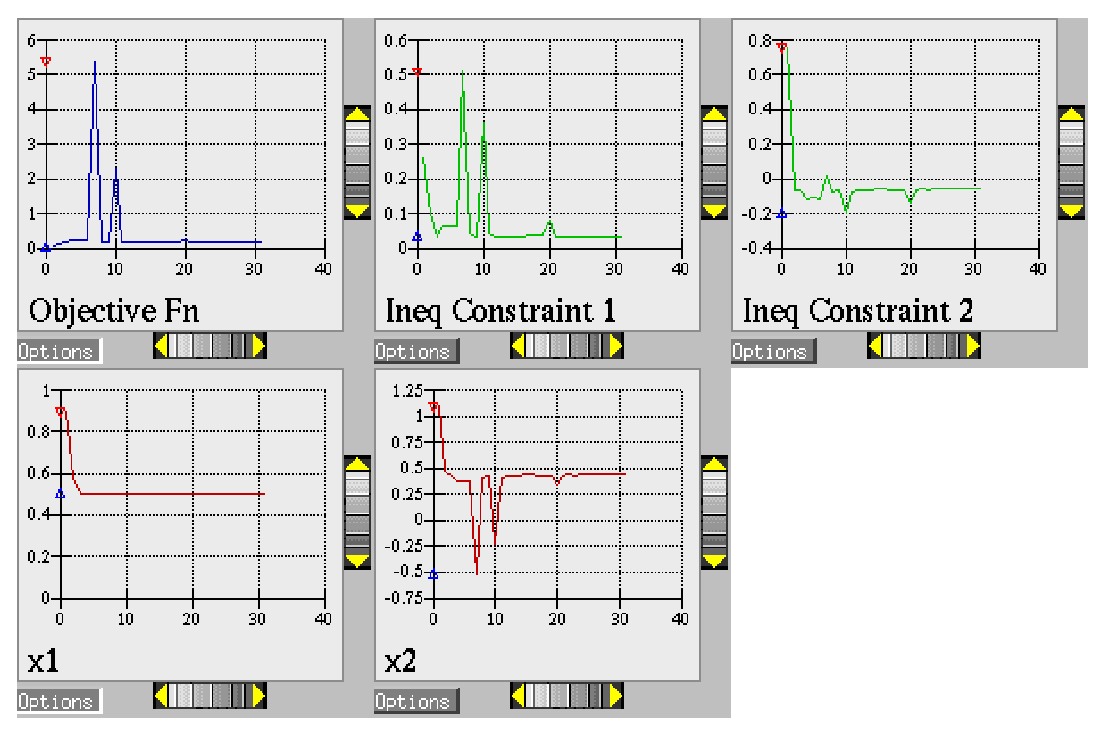
\includegraphics[width=\textwidth]{images/textbook_opt_hist}\\
  (a)\\
  \qquad\\
  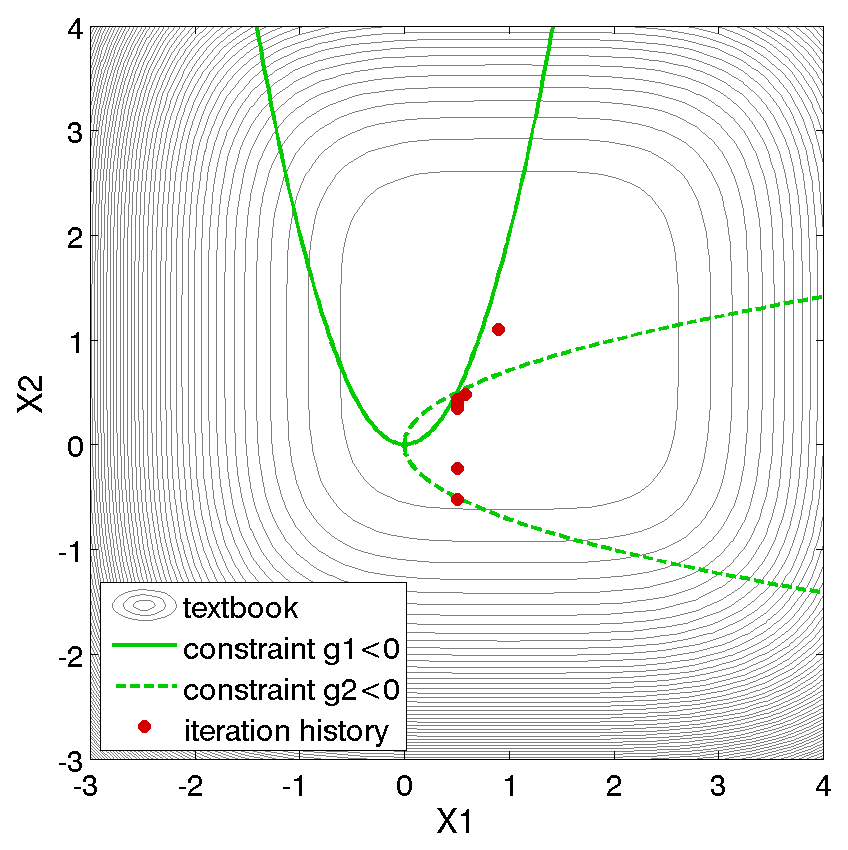
\includegraphics[height=2.5in]{images/textbook_history} \\
  (b)
  \end{tabular}
  \caption{Textbook gradient-based constrained optimization example:
    (a) screen capture of the DAKOTA graphics shows how the objective
    function was reduced during the search for a feasible design point
    and (b) iteration history (iterations marked by solid dots).}
  \label{additional:textbook_grad_constr_graphics}
\end{figure}

\subsubsection{Least Squares Optimization}\label{additional:textbook:least}

This test problem may also be used to exercise least squares
solution methods by modifying the problem formulation to:
\begin{equation}
\texttt{minimize } (f)^2+(g_1)^2+(g_2)^2 \label{additional:tbls}
\end{equation}

This modification is performed by simply changing the responses
specification for the three functions from
\texttt{num\_objective\_functions = 1} and
\texttt{num\_nonlinear\_inequality\_constraints = 2} to \\
\texttt{num\_least\_squares\_terms = 3}. Note that the two problem
formulations are not equivalent and have different solutions.

Another way to exercise the least squares methods which would be
equivalent to the optimization formulation would be to select the
residual functions to be $(x_{i}-1)^2$. However, this formulation
requires modification to \texttt{Dakota/test/text\_book.C} and will
not be presented here. Equation~\ref{additional:tbls}, on the other
hand, can use the existing \texttt{text\_book.C} without modification.
Refer to Section~\ref{additional:rosenbrock} for an example of
minimizing the same objective function using both optimization and
least squares approaches.

The solution for the least squares problem given in 
Equation~\ref{additional:tbls} is:
\begin{eqnarray*}
    x_1 &=& 0.566 \\
    x_2 &=& 0.566
\end{eqnarray*}
with the residual functions equal to
\begin{eqnarray*}
      f^{\ast} &=& 0.0713 \\
    g_1^{\ast} &=& 0.0371 \\
    g_2^{\ast} &=& 0.0371
\end{eqnarray*}
and a minimal sum of the squares of $0.00783$.

This study requires selection of \texttt{num\_least\_squares\_terms = 3} 
in the responses specification and selection of either 
\texttt{optpp\_g\_newton}, \texttt{nlssol\_sqp}, or \texttt{nl2sol} in 
the method specification.

\subsubsection{Other Optimization Methods}

% The \texttt{dakota\_textbook.in} file provided in the
% \texttt{Dakota/examples/tutorial} directory selects a \\
% \texttt{conmin\_mfd}
% \texttt{dot\_mmfd} 
% optimizer to perform constrained minimization using
% the \texttt{text\_book} simulator. 
Additional gradient-based methods
that can be used include methods from the
DOT, 
%CONMIN, 
NPSOL, NLPQL, and OPT++ packages.
In addition the unconstrained least squares formulation of
Equation~\ref{additional:tbls} can be solved using OPT++ Gauss-Newton,
NLSSOL, and NL2SOL methods.

A hybrid optimization strategy can also be demonstrated on the
\texttt{text\_book} problem. The \texttt{dakota\_hybrid.in} file
provided in {\tt Dakota/examples/methods} starts with a
\texttt{coliny\_ea} solution which feeds its best point into a
\texttt{coliny\_pattern\_search} optimization which feeds its best
point into \texttt{optpp\_newton}. While this approach is overkill for
such a simple problem, it is useful for demonstrating the coordination
between multiple methods in the hybrid strategy.

In addition, \texttt{Dakota/test/dakota\_textbook\_3pc.in}
demonstrates the use of a 3-piece interface to perform the parameter
to response mapping, and \texttt{Dakota/test/dakota\_textbook\_lhs.in}
demonstrates the use of Latin hypercube Monte Carlo sampling for
assessing probability of failure as measured by specified response
levels.

\subsubsection{Reliability Methods}\label{additional:textbook:examples:reliability}

Reliability methods provide an alternative approach to uncertainty
quantification which can be less computationally demanding than
sampling techniques. Reliability methods for uncertainty
quantification are based on probabilistic approaches that compute
approximate response function distribution statistics based on
specified uncertain variable distributions. These response statistics
include response mean, response standard deviation, and cumulative or
complementary cumulative distribution functions (CDF/CCDF). These
methods are often more efficient at computing statistics in the tails
of the response distributions (events with low probability) than
sampling based approaches since the number of samples required to
resolve a low probability can be prohibitive.

Figure~\ref{additional:textbook_mv} shows the DAKOTA input file for an
example problem that demonstrates the simplest reliability method,
called the mean value method (also referred to as the Mean Value First
Order Second Moment method). It is specified with method keyword
\texttt{local\_reliability}. This method calculates the mean and
variance of the response function based on information about the mean
and variance of the inputs and gradient information at the mean of the
inputs. The mean value method is extremely cheap computationally (only
five runs were required for the textbook function), but can be quite
inaccurate, especially for nonlinear problems and/or problems with
uncertain inputs that are significantly non-normal. More detail on the
mean value method can be found in the Local Reliability Methods
section of the DAKOTA Theory Manual~\cite{TheoMan}, and more detail on
reliability methods in general (including the more advanced methods)
is found in Section~\ref{uq:reliability}.

Example output from the mean value method is displayed in 
Figure~\ref{additional:results_mv}. Note that since the mean of both inputs
is 1, the mean value of the output for response 1 is zero. 
However, the mean values of the constraints are both 0.5. 
The mean value results indicate that variable x1 is more 
important in constraint 1 while x2 is more important in constraint 2, 
which is the case based on Equation~\ref{additional:textbook_f}.

This DAKOTA input file is executed using the following command:
\begin{small}
\begin{verbatim}
         dakota dakota_mv.in > mv.out
\end{verbatim}
\end{small}
See the file \texttt{mv.out.sav} in \texttt{Dakota/examples/tutorial} 
for comparison with results from DAKOTA. 

\begin{figure}[ht!]
  \centering
  \begin{bigbox}
    \begin{small}
      \verbatimtabinput[8]{dakota_mv.in}
    \end{small}
  \end{bigbox}
  \caption{Mean Value Reliability Method: the DAKOTA input file.}
  \label{additional:textbook_mv}
\end{figure}

\begin{figure}
\centering
\begin{bigbox}
\begin{small}
\begin{verbatim}
-----------------------------------------------------------------
MV Statistics for response_fn_1:
  Approximate Mean Response                  =  0.0000000000e+00
  Approximate Standard Deviation of Response =  0.0000000000e+00
  Importance Factors not available.
MV Statistics for response_fn_2:
  Approximate Mean Response                  =  5.0000000000e-01
  Approximate Standard Deviation of Response =  1.0307764064e+00
  Importance Factor for variable TF1ln       =  9.4117647059e-01
  Importance Factor for variable TF2ln       =  5.8823529412e-02
MV Statistics for response_fn_3:
  Approximate Mean Response                  =  5.0000000000e-01
  Approximate Standard Deviation of Response =  1.0307764064e+00
  Importance Factor for variable TF1ln       =  5.8823529412e-02
  Importance Factor for variable TF2ln       =  9.4117647059e-01
-----------------------------------------------------------------
\end{verbatim}
\end{small}
\end{bigbox}
\caption{Results of the Mean Value Method on the Textbook Function}
\label{additional:results_mv}
\end{figure}



\section{Rosenbrock Examples}\label{additional:rosenbrock}

The Rosenbrock function~\cite{Gil81} is a well known benchmark problem
for optimization algorithms. Its standard two-dimensional formulation
can be stated as
\begin{equation}
\texttt{minimize } f=100(x_2-x_1^2)^2+(1-x_1)^2 \label{additional:rosenstd}
\end{equation}
Two $n$-dimensional formulations are present in the literature.
First, \cite{Noc99} formulates an ``extended Rosenbrock'' as:
\begin{equation}
f = \sum_{i=1}^{n/2} \left[ \alpha (x_{2i}-x_{2i-1}^2)^2+(1-x_{2i-1})^2 \right]
\label{additional:rosenexd}
\end{equation}
Second, \cite{Sch87} formulates a ``generalized Rosenbrock'' as:
\begin{equation}
f = \sum_{i=1}^{n-1} \left[ 100 (x_{i+1}-x_i^2)^2+(1-x_i)^2 \right]
\label{additional:rosengen}
\end{equation}
These formulations are not currently supported in DAKOTA's
system/fork interfaces, but are supported in the direct interface.

%\begin{equation}
%f = \sum_{i=1}^{n/2} \left[ e^{-x^2_{2i-1}} + 10 e^{-x^2_{2i}} \right]
%\label{additional:gerstner_aniso1}
%\end{equation}
%\begin{equation}
%f = exp\left(-\sum_{i=1}^{n/2} \left[ 10 x^2_{2i-1} + 5 x^2_{2i} \right]\right)
%\label{additional:gerstner_aniso3}
%\end{equation}

Surface and contour plots for this function have been shown previously
in Figure~\ref{tutorial:rosenbrock_prob}. This example problem
may also be used to exercise least squares solution methods by
recasting the problem formulation into:
\begin{equation}
\texttt{minimize } f = (f_1)^2+(f_2)^2 \label{additional:rosenls}
\end{equation}
where
\begin{equation}
f_1 = 10 (x_2 - x_1^2) \label{additional:rosenr1}
\end{equation}
and
\begin{equation}
f_2 = 1 - x_1 \label{additional:rosenr2}
\end{equation}
are residual terms. In this case (unlike the least squares
modification in Section~\ref{additional:textbook}), the two problem
formulations are equivalent and have identical solutions.

\subsection{Examples}\label{additional:rosenbrock:examples}

\subsubsection{Vector Parameter Study}\label{additional:rosenbrock:examples:vector}

In addition to the multidimensional parameter study, DAKOTA can
perform a vector parameter study, i.e., a parameter study between any
two design points in an \emph{n}-dimensional parameter space.

An input file for the vector parameter study is shown in Figure~
\ref{additional:rosenbrock_vector}. The primary differences
between this input file and the previous input file are found in the
\emph{variables} and \emph{method} sections. In the variables section,
the keywords for the bounds are removed and replaced with the keyword
\texttt{initial\_point} that specifies the starting point for the
parameter study. In the method section, the
\texttt{vector\_parameter\_study} keyword is used. The
\texttt{final\_point} keyword indicates the stopping point for the
parameter study, and \texttt{num\_steps} specifies the number of steps
taken between the initial and final points in the parameter study.

\begin{figure}[ht!]
  \centering
  \begin{bigbox}
    \begin{small}
      \verbatimtabinput[8]{dakota_rosenbrock_vector.in}
    \end{small}
  \end{bigbox}
  \caption{Rosenbrock vector parameter study example: the DAKOTA input
  file.}
  \label{additional:rosenbrock_vector}
\end{figure}

The vector parameter study example problem is executed using the command
\begin{small}
\begin{verbatim}
    dakota dakota_rosenbrock_vector.in > vector.out
\end{verbatim}
\end{small}

Figure~\ref{additional:rosenbrock_vector_graphics}(a) shows the
graphics output created by DAKOTA. For this study, the simple DAKOTA
graphics are more useful for visualizing the
results. Figure~\ref{additional:rosenbrock_vector_graphics}(b)
shows the locations of the 11 sample points generated in this study.
It is evident from these figures that the parameter study starts
within the banana-shaped valley, marches up the side of the hill, and
then returns to the valley. The output file \texttt{vector.out.sav} is
provided in the \texttt{Dakota/examples/tutorial} directory.

In addition to the vector and multidimensional examples shown, DAKOTA
also supports list and centered parameter study methods. Refer to
Chapter~\ref{ps} for additional information.

\begin{figure}[htp!]
  \centering
  \begin{tabular}{c}
  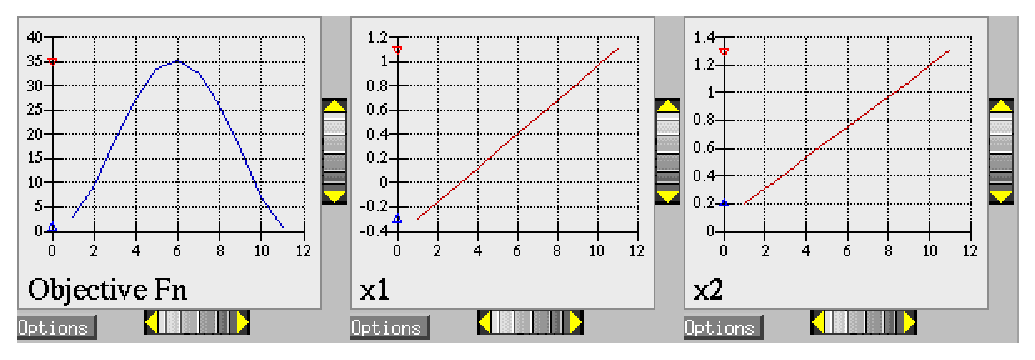
\includegraphics[width=\textwidth]{images/dak_graphics_vector}\\
  (a)\\
  \qquad\\
  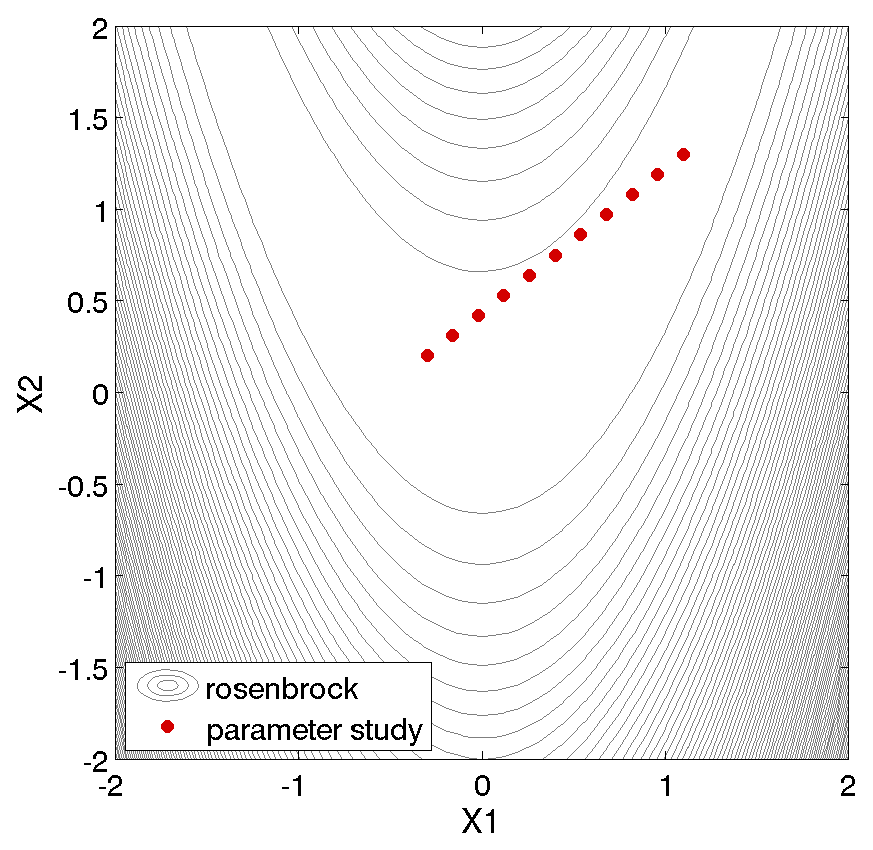
\includegraphics[height=2.5in]{images/rosen_vect_pts} \\
  (b)
  \end{tabular}
  \caption{Rosenbrock vector parameter study example: (a) screen
    capture of the DAKOTA graphics and (b) location of the design
    points (dots) evaluated.}
  \label{additional:rosenbrock_vector_graphics}
\end{figure}

\subsubsection{Nonlinear Least Squares Methods for Optimization}\label{additional:rosenbrock:examples:nonlinear}

Least squares methods are often used for calibration or parameter
estimation, that is, to seek parameters maximizing agreement of models
with experimental data. Both the Rosenbrock and textbook example
problems can be formulated as least-squares minimization problems (see
Section~\ref{additional:textbook} and
Section~\ref{additional:rosenbrock}). For example, the Rosenbrock
problem can be cast as:
\begin{equation}
\texttt{minimize } (f_1)^2 + (f_2)^2
\end{equation}

where $f_1 = 10(x_2-x_1^2)$ and $f_2 = (1-x_1)$. When
using a least-squares approach to minimize a function, each of the
least-squares terms $f_1, f_2,\ldots$ is driven toward zero. This
formulation permits the use of specialized algorithms that can be more
efficient than general purpose optimization algorithms. See
Chapter~\ref{nls} for more detail on the algorithms used for least-squares
minimization, as well as a discussion on the types of
engineering design problems (e.g., parameter estimation) that can make
use of the least-squares approach.

Figure~\ref{additional:rosenbrock_nls} is a listing of the DAKOTA input
file \texttt{dakota\_rosenbrock\_ls.in}. This differs from the input
file shown in Figure~\ref{tutorial:rosenbrock_grad} in several key
areas. The responses block of the input file uses the keyword
\texttt{calibration\_terms = 2} instead of
\texttt{objective\_functions = 1}.
%The keywords in the interface block show that the Unix fork method
%is used to run the C++ analysis code named \texttt{rosenbrock}.
The method block of the input file shows that the NL2SOL
algorithm~\cite{Den81} (\texttt{nl2sol}) is used in this example. (The
Gauss-Newton, NL2SOL, and NLSSOL SQP algorithms are currently
available for exploiting the special mathematical structure of least
squares minimization problems).

\begin{figure}[ht!]
  \centering
  \begin{bigbox}
    \begin{small}
      \verbatimtabinput[8]{dakota_rosenbrock_ls.in}
    \end{small}
  \end{bigbox}
  \caption{Rosenbrock nonlinear least squares example: the DAKOTA input file.}
  \label{additional:rosenbrock_nls}
\end{figure}

The input file listed in Figure~\ref{additional:rosenbrock_nls} is
executed using the command:
\begin{small}
\begin{verbatim}
    dakota dakota_rosenbrock_ls.in > leastsquares.out
\end{verbatim}
\end{small}

The file \texttt{leastsquares.out.sav} is included
\texttt{Dakota/examples/tutorial} for comparison purposes. The
optimization results at the end of this file show that the least
squares minimization approach has found the same optimum design point,
$(x1,x2) = (1.0,1.0)$, as was found using the conventional
gradient-based optimization approach. The iteration history of the
least squares minimization is given in
Figure~\ref{additional:rosenbrock_nls_graphics}, and shows that 14
function evaluations were needed for convergence. In this example the
least squares approach required about half the number of function
evaluations as did conventional gradient-based optimization.
In many cases a good least squares algorithm will converge more rapidly
in the vicinity of the solution.

\begin{figure}[ht!]
  \centering
  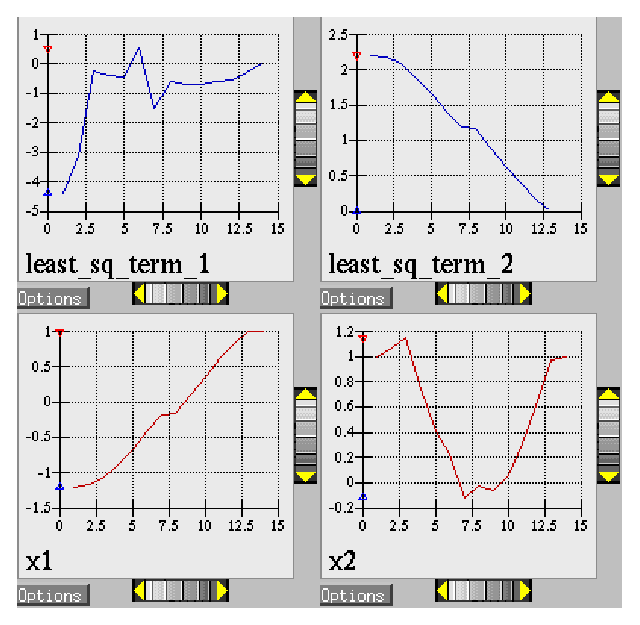
\includegraphics[height=4in]{images/nonlin_paramest_hist}
  \caption{Rosenbrock nonlinear least squares example: iteration
    history for least squares terms $f_1$ and $f_2$.}
  \label{additional:rosenbrock_nls_graphics}
\end{figure}

\subsubsection {Least Squares Optimization}\label{additional:rosenbrock:examples:lsq}

In the \texttt{Dakota/test} directory, the \texttt{rosenbrock}
executable (compiled from \texttt{rosenbrock.C}) checks the number of
response functions passed in the parameters file and returns either an
objective function (as computed from
Equation~\ref{additional:rosenstd}) for use with optimization methods
or two least squares terms (as computed from
Equations~\ref{additional:rosenr1}-\ref{additional:rosenr2}) for use
with least squares methods. Both cases support analytic gradients of
the function set with respect to the design variables. The
\texttt{dakota\_rosenbrock.in} input file can be used to solve both
problems by toggling settings in the method and responses
specifications. To run the optimization solution, select
\texttt{num\_objective\_functions = 1} in the responses specification,
and select an optimizer (e.g., \texttt{optpp\_q\_newton}) in the
method specification, e.g., as shown in \\ {\tt
Dakota/examples/methods/dakota\_addtnl\_rosen\_opt.in}:
\begin{center}
  \begin{small}
    \begin{bigbox}
      \verbatimtabinput[8]{dakota_addtnl_rosen_opt.in}
    \end{bigbox}
  \end{small}
\end{center}

To run the least squares solution, the responses specification is
changed to \texttt{num\_least\_squares\_terms = 2} and the method
specification is changed to a least squares method, e.g.,
\texttt{optpp\_g\_newton}, as shown in {\tt
Dakota/examples/methods/dakota\_addtnl\_rosen\_ls.in}:
\begin{center}
  \begin{small}
    \begin{bigbox}
      \verbatimtabinput[8]{dakota_addtnl_rosen_ls.in}
    \end{bigbox}
  \end{small}
\end{center}

\subsubsection{Nongradient-based Optimization via Pattern Search}\label{additional:rosenbrock:examples:nongradient1}

In addition to gradient-based optimization algorithms, DAKOTA also
contains a variety of nongradient-based algorithms. One particular
nongradient-based algorithm for local optimization is known as pattern
search (see Chapter~\ref{introduction} for a discussion of local
versus global optimization). The DAKOTA input file shown in
Figure~\ref{additional:rosenbrock_patternsearch} applies a pattern
search method to minimize the Rosenbrock function. While this
provides for an interesting comparison to the previous example
problems in this chapter, the Rosenbrock function is not the best test
case for a pattern search method. That is, pattern search methods are
better suited to problems where the gradients are too expensive to
evaluate, inaccurate, or nonexistent --- situations common among many
engineering optimization problems. It also should be noted that
nongradient-based algorithms generally are applicable only to
unconstrained or bound-constrained optimization problems, although the
inclusion of general linear and nonlinear constraints in
nongradient-based algorithms is an active area of research in the
optimization community. For most users who wish to use
nongradient-based algorithms on constrained optimization problems, the
easiest route is to create a penalty function, i.e., a composite
function that contains the objective function and the constraints,
external to DAKOTA and then optimize on this penalty function. Most
optimization textbooks will provide guidance on selecting and using
penalty functions.

The DAKOTA input file shown in
Figure~\ref{additional:rosenbrock_patternsearch} is similar to the
input file for the gradient-based optimization, except it has a
different set of keywords in the method block of the input file, and
the gradient specification in the responses block has been changed
to \texttt{no\_gradients}. The pattern search optimization algorithm
used is part of the SCOLIB library~\cite{Har06}. See the DAKOTA
Reference Manual~\cite{RefMan} for more information on the
\emph{methods} block commands that can be used with SCOLIB
algorithms.

\begin{figure}[ht!]
  \centering
  \begin{bigbox}
    \begin{small}
      \verbatimtabinput[8]{dakota_rosenbrock_ps_opt.in}
    \end{small}
  \end{bigbox}
  \caption{Rosenbrock pattern search optimization example: the DAKOTA input file.}
  \label{additional:rosenbrock_patternsearch}
\end{figure}

This DAKOTA input file is executed using the following command:
\begin{small}
\begin{verbatim}
    dakota dakota_rosenbrock_ps_opt.in > ps_opt.out
\end{verbatim}
\end{small}

The file \texttt{ps\_opt.out.sav} is included in the
\texttt{Dakota/examples/tutorial} directory. For this run, the
optimizer was given an initial design point of $(x_1,x_2)
  = (0.0,0.0)$ and was limited to 2000 function evaluations. In this
case, the pattern search algorithm stopped short of the optimum at
$(x_1,x_2) = (1.0,1,0)$, although it was making progress
in that direction when it was terminated. (It would have
reached the minimum point eventually.)

The iteration history is provided in Figures~
\ref{additional:rosenbrock_patternsearch_graphics}(a) and (b), which show
the locations of the function evaluations used in the pattern search
algorithm.
Figure~\ref{additional:rosenbrock_patternsearch_graphics}(c)
provides a close-up view of the pattern search function evaluations
used at the start of the algorithm. The coordinate pattern is clearly
visible at the start of the iteration history, and the decreasing size
of the coordinate pattern is evident at the design points move toward
$(x_1,x_2) = (1.0,1.0)$.

\begin{figure}[ht!]
  \centering
  \begin{tabular}{cc}
  \multicolumn{2}{c}
	      {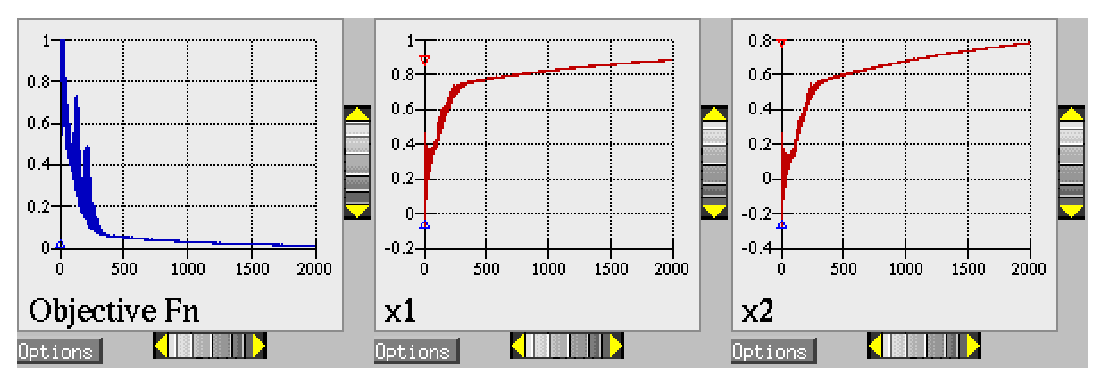
\includegraphics[width=\textwidth]{images/dak_graphics_ps_opt}}\\
  \multicolumn{2}{c}{(a)}\\
  \qquad\\
  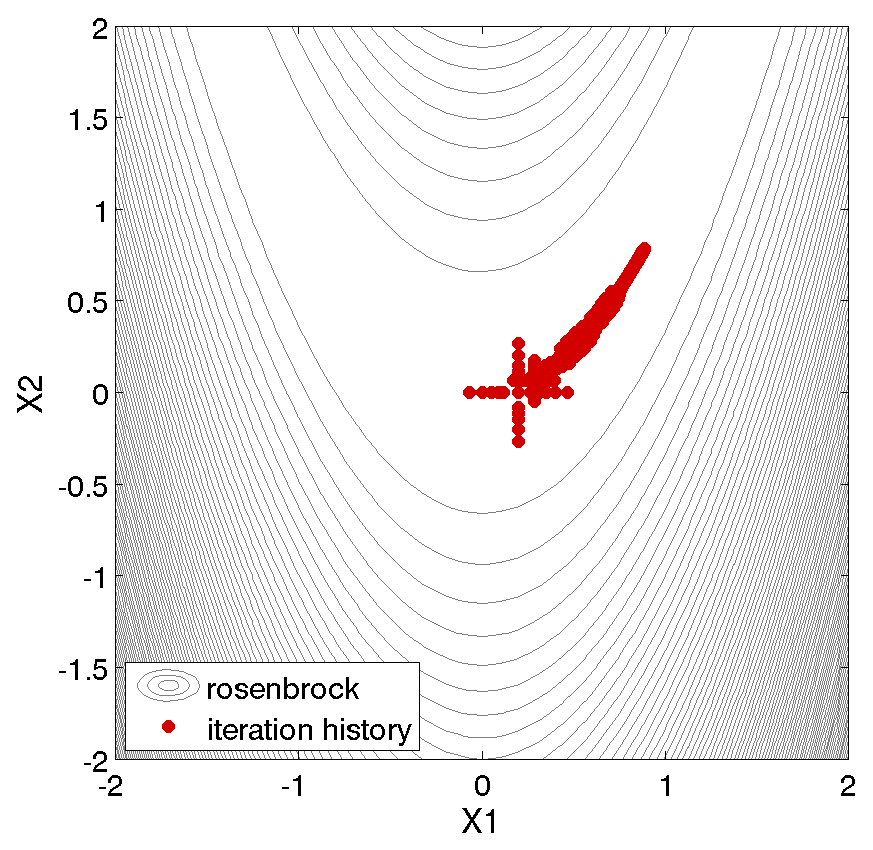
\includegraphics[height=2.5in]{images/rosen_ps_opt_pts} &
  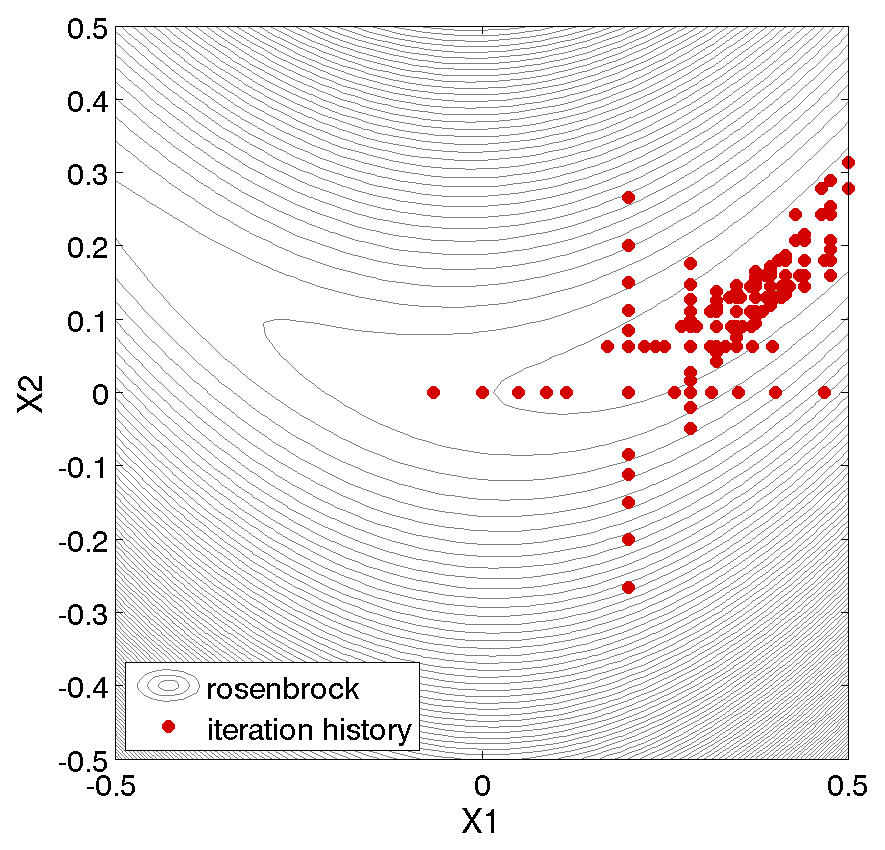
\includegraphics[height=2.5in]{images/rosen_ps_opt_pts2} \\
  (b) & (c)
  \end{tabular}
  \caption{Rosenbrock pattern search optimization example: (a) screen
    capture of the DAKOTA graphics, (b) sequence of design points
    (dots) evaluated and (c) close-up view illustrating the shape of
    the coordinate pattern used. }
  \label{additional:rosenbrock_patternsearch_graphics}
\end{figure}

While pattern search algorithms are useful in many optimization
problems, this example shows some of the drawbacks to this algorithm.
While a pattern search method may make good initial progress towards
an optimum, it is often slow to converge. On a smooth, differentiable
function such as Rosenbrock's function, a nongradient-based method
will not be as efficient as a gradient-based method. However, there
are many engineering design applications where gradient information is
inaccurate or unavailable, which renders gradient-based optimizers
ineffective. Thus, pattern search algorithms (and other
nongradient-based algorithms such as genetic algorithms as discussed in the
next section) are often good choices in complex engineering applications
when the quality of gradient data is suspect.

\subsubsection{Nongradient-based Optimization via Evolutionary Algorithm}\label{additional:rosenbrock:examples:nongradient2}

In contrast to pattern search algorithms, which are local optimization
methods, evolutionary algorithms (EA) are global optimization
methods. As was described above for the pattern search algorithm, the
Rosenbrock function is not an ideal test problem for showcasing the
capabilities of evolutionary algorithms. Rather, EAs are best suited
to optimization problems that have multiple local optima, and where
gradients are either too expensive to compute or are not readily available.

Evolutionary algorithms are based on Darwin's theory of survival of
the fittest. The EA algorithm starts with a randomly selected
population of design points in the parameter space, where the values
of the design parameters form a ``genetic string,'' analogous
to DNA in a biological system, that uniquely represents each design
point in the population. The EA then follows a sequence of
generations, where the best design points in the population (i.e.,
those having low objective function values) are considered to be the
most ``fit'' and are allowed to survive and reproduce. The EA
simulates the evolutionary process by employing the mathematical
analogs of processes such as natural selection, breeding, and
mutation. Ultimately, the EA identifies a design point (or a family of
design points) that minimizes the objective function of the
optimization problem. An extensive discussion of EAs is beyond the
scope of this text, but may be found in a variety of sources (cf.,
~\cite{Haf92} pp. 149-158;~\cite{Gol89}). Currently, the EAs available
in DAKOTA include a genetic algorithm for problems involving discrete
variables and an evolution strategy with self-adaptation for problems
with continuous variables. Details of these algorithms are given in
the DAKOTA Reference Manual~\cite{RefMan}. The SCOLIB library, which
provides the EA software that has been linked into DAKOTA, is
described in~\cite{Har06}.

\begin{figure}[ht!]
  \centering
  \begin{bigbox}
    \begin{small}
      \verbatimtabinput[8]{dakota_rosenbrock_ea_opt.in}
    \end{small}
  \end{bigbox}
  \caption{Rosenbrock evolutionary algorithm optimization example: the
  DAKOTA input file.}
  \label{additional:rosenbrock_ea}
\end{figure}

Figure~\ref{additional:rosenbrock_ea} shows a DAKOTA input file that
uses an EA to minimize the Rosenbrock function. For this
example the EA has a population size of 50. At the start of the first
generation, a random number generator is used to select 50 design
points that will comprise the initial population. \emph{[A specific
  seed value is used in this example to generate repeatable results,
  although, in general, one should use the default setting which
  allows the EA to choose a random seed.]} A two-point crossover
technique is used to exchange genetic string values between the
members of the population during the EA breeding process. The result
of the breeding process is a population comprised of the 10 best
``parent'' design points (elitist strategy) plus 40 new ``child''
design points. The EA optimization process will be terminated after
either 100 iterations (generations of the EA) or 2,000 function
evaluations. The EA software available in DAKOTA provides the user
with much flexibility in choosing the settings used in the
optimization process. See~\cite{RefMan} and~\cite{Har06} for details on these
settings.

The following command runs DAKOTA on the input file:
\begin{small}
\begin{verbatim}
    dakota dakota_rosenbrock_ea_opt.in > ea_opt.out
\end{verbatim}
\end{small}

A corresponding output file named \texttt{ea\_opt.out.sav} appears in
\texttt{Dakota/examples/tutorial}. The EA optimization results
printed at the end of this file show that the best design point found
was $(x_1,x_2) = (0.98,0.95)$. The file
\texttt{ea\_tabular.dat.sav} provides a listing of the design
parameter values and objective function values for all 2,000 design
points evaluated during the running of the EA. Figure~
\ref{additional:rosenbrock_ea_graphics}(a) shows the population of
50 randomly selected design points that comprise the first generation
of the EA, and Figure~\ref{additional:rosenbrock_ea_graphics}(b)
shows the final population of 50 design points, where most of the 50
points are clustered near $(x_1,x_2) = (0.98,0.95)$.

\begin{figure}[hbt!]
  \centering
  \begin{tabular}{cc}
  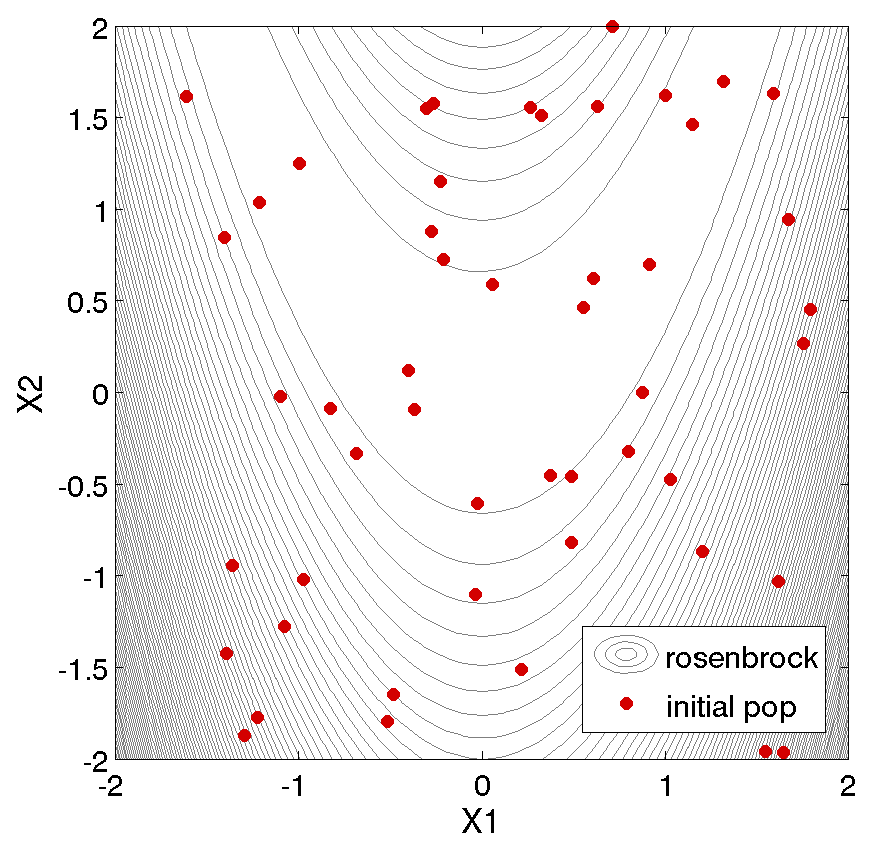
\includegraphics[height=2.5in]{images/rosen_ea_init} &
  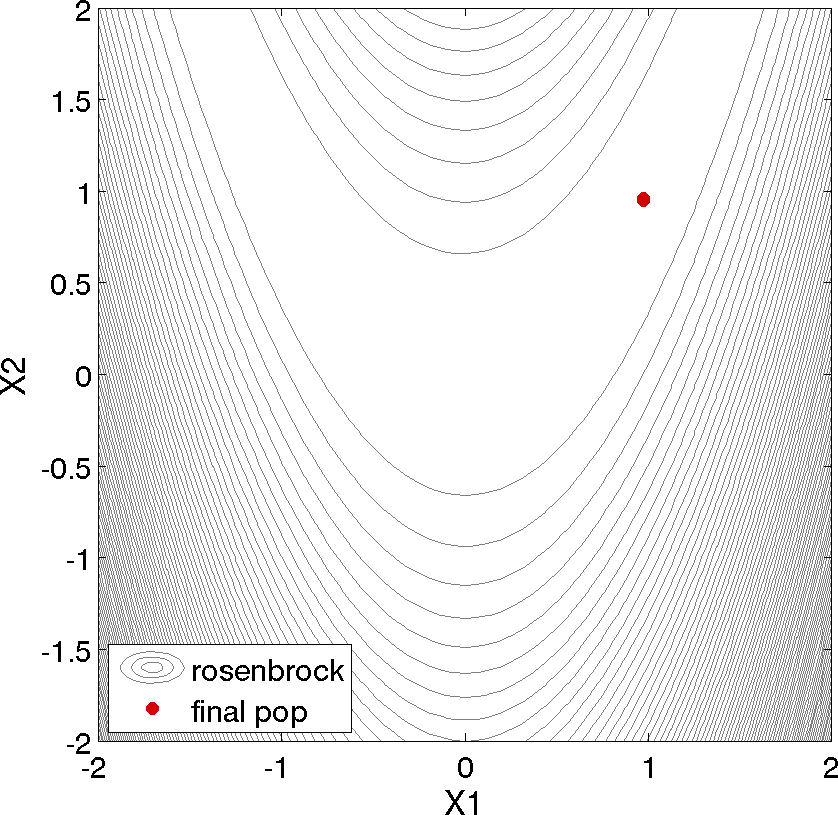
\includegraphics[height=2.5in]{images/rosen_ea_final} \\
  (a) & (b)
  \end{tabular}
  \caption{Rosenbrock evolutionary algorithm optimization example: 50
    design points in the (a) initial and (b) final populations
    selected by the evolutionary algorithm. }
  \label{additional:rosenbrock_ea_graphics}
\end{figure}

As described above, an EA is not well-suited to an optimization
problem involving a smooth, differentiable objective such as the
Rosenbrock function. Rather, EAs are better suited to optimization
problems where conventional gradient-based optimization fails, such as
situations where there are multiple local optima and/or gradients are
not available. In such cases, the computational expense of an EA is
warranted since other optimization methods are not applicable or
impractical. In many optimization problems, EAs often quickly identify
promising regions of the design space where the global minimum may be
located. However, an EA can be slow to converge to the optimum. For
this reason, it can be an effective approach to combine the global
search capabilities of a EA with the efficient local search of a
gradient-based algorithm in a \emph{hybrid optimization} strategy. In
this approach, the optimization starts by using a few iterations of a
EA to provide the initial search for a good region of the parameter
space (low objective function and/or feasible constraints), and then
it switches to a gradient-based algorithm (using the best design point
found by the EA as its starting point) to perform an efficient local
search for an optimum design point. More information on this hybrid
approach is provided in Chapter~\ref{strat}.

In addition to the evolutionary algorithm capabilities in the
\texttt{coliny\_ea} method, there is a single-objective genetic algorithm
method called \texttt{soga}.
%The major differences are that
%\texttt{soga} allows a warm start (e.g., you can read in starting
%solutions from a file), and it allows one to specify a mix of
%continuous and discrete design variables.
For more information on \texttt{soga}, see Chapter~\ref{opt}.

\subsubsection{Uncertainty Quantification using Polynomial Chaos Expansions}\label{additional:rosenbrock:examples:pce}
The term ``Polynomial Chaos'' refers to the representation of a stochastic 
process as a polynomial expansion in random (or stochastic) variables. This 
representation acts as a response surface that maps stochastic inputs to 
stochastic outputs. Desired statistics can then be obtained from the 
response surface either analytically or by re-sampling the fast surrogate.
Exponential convergence of the error with increasing polynomial order can 
be obtained by using (an) orthogonal polynomial series whose weighting 
function(s) is/are the probability density functions of the stochastic 
inputs. Coefficients in the Chaos expansion are determined through
orthogonal projection. For non-intrusive implementations, such as in DAKOTA,
numerical integration via quadrature or cubature is used to evaluate the 
orthogonal projections. Additional details regarding the method are 
provided in Section~\ref{uq:expansion}.

A typical DAKOTA input file for performing an uncertainty
quantification using polynomial chaos expansions is shown in
Figure~\ref{additional:pce}, \texttt{dakota\_pce.in}.
In this example, we compute CDF
probabilities for six response levels of Rosenbrock's function. Since
Rosenbrock is a fourth order polynomial and we employ a fourth-order
expansion using an optimal basis (Legendre for uniform random
variables), we can readily obtain a polynomial expansion which exactly
matches the Rosenbrock function. In this example, we select Gaussian
quadratures using an anisotropic approach (fifth-order quadrature in
$x_1$ and third-order quadrature in $x_2$), resulting in a total of
15 function evaluations to compute the PCE coefficients.

\begin{figure}
  \centering
  \begin{bigbox}
    \begin{small}
      \verbatimtabinput[8]{dakota_pce.in}
    \end{small}
  \end{bigbox}
\caption{DAKOTA input file for performing UQ using polynomial chaos expansions.}
\label{additional:pce}
\end{figure}

The tensor product quadature points upon which the expansion is calculated 
are shown in Figure~\ref{additional:rosen_pce_points}. 
The tensor product generates
all combinations of values from each individual dimension: it is an 
all-way pairing of points.

\begin{figure}[ht!]
  \centering
  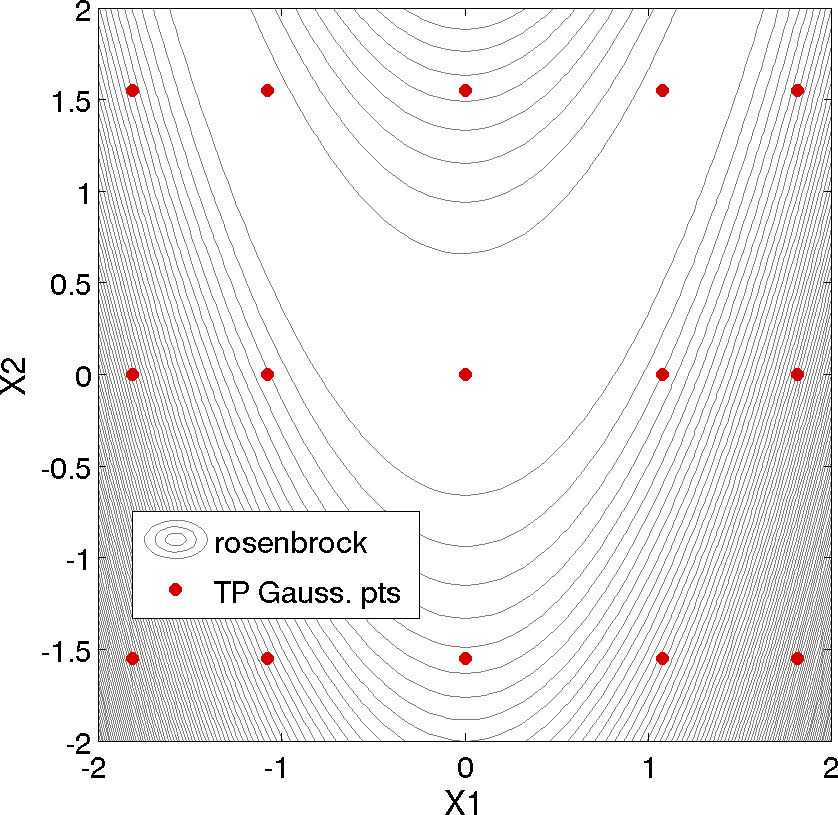
\includegraphics[height=2.5in]{images/rosen_pce_pts}
  \caption{Rosenbrock polynomial chaos example: tensor product quadrature points.}
  \label{additional:rosen_pce_points}
\end{figure}

Once the expansion coefficients have been calculated, some statistics
are available analytically and others must be evaluated numerically.
For the numerical portion, the input file specifies the use of 10000
samples, which will be evaluated on the expansion to compute the CDF
probabilities. In Figure~\ref{additional:pce_out}, excerpts from the results
summary are presented, where we first see a summary of the PCE
coefficients which exactly reproduce Rosenbrock for a Legendre
polynomial basis. The analytic statistics for mean, standard
deviation, and COV are then presented. For example, the mean is 455.66 
and the standard deviation is 606.56. The moments are followed 
by global sensitivity indices (Sobol indices).This example shows that variable 
x1 has the largest main effect (0.497) as compared with variable 
x2 (0.296) or the interaction between x1 and x2 (0.206). 
After the global sensitivity indices, the local, analytic random 
variable sensitivities are presented, evaluated at the mean values.
Finally, we see the numerical results for the CDF probabilities based
on 10000 samples performed on the expansion. For example, 
the probability that the Rosenbrock function is less than 100 
over these two uncertain variables is 0.342. Note that this is a very similar 
estimate to what was obtained using 200 Monte Carlo samples, with 
fewer function evaluations.
\begin{figure}
\centering
\begin{bigbox}
%\begin{footnotesize}
\begin{scriptsize}
\begin{verbatim}
Polynomial Chaos coefficients for response_fn_1:
        coefficient   u1   u2
        ----------- ---- ----
   4.5566666667e+02   P0   P0
  -4.0000000000e+00   P1   P0
   9.1695238095e+02   P2   P0
  -9.9475983006e-14   P3   P0
   3.6571428571e+02   P4   P0
  -5.3333333333e+02   P0   P1
  -3.9968028887e-14   P1   P1
  -1.0666666667e+03   P2   P1
  -3.3573144265e-13   P3   P1
   1.2829737273e-12   P4   P1
   2.6666666667e+02   P0   P2
   2.2648549702e-13   P1   P2
   4.8849813084e-13   P2   P2
   2.8754776338e-13   P3   P2
  -2.8477220582e-13   P4   P2
-------------------------------------------------------------------
Statistics derived analytically from polynomial expansion:

Moment-based statistics for each response function:
                            Mean           Std Dev          Skewness          Kurtosis
response_fn_1
  expansion:    4.5566666667e+02  6.0656024184e+02
  numerical:    4.5566666667e+02  6.0656024184e+02  1.9633285271e+00  3.3633861456e+00

Covariance among response functions:
[[  3.6791532698e+05 ]] 

Local sensitivities for each response function evaluated at uncertain variable means:
response_fn_1:
 [ -2.0000000000e+00  2.4055757386e-13 ] 

Global sensitivity indices for each response function:
response_fn_1 Sobol indices:
                                  Main             Total
                      4.9746891383e-01  7.0363551328e-01 x1
                      2.9636448672e-01  5.0253108617e-01 x2
                           Interaction
                      2.0616659946e-01 x1 x2 

Statistics based on 10000 samples performed on polynomial expansion:

Probability Density Function (PDF) histograms for each response function:
PDF for response_fn_1:
          Bin Lower          Bin Upper      Density Value
          ---------          ---------      -------------
   6.8311107124e-03   1.0000000000e-01   2.0393073423e-02
   1.0000000000e-01   1.0000000000e+00   1.3000000000e-02
   1.0000000000e+00   5.0000000000e+01   4.7000000000e-03
   5.0000000000e+01   1.0000000000e+02   1.9680000000e-03
   1.0000000000e+02   5.0000000000e+02   9.2150000000e-04
   5.0000000000e+02   1.0000000000e+03   2.8300000000e-04
   1.0000000000e+03   3.5755437782e+03   5.7308286215e-05

Level mappings for each response function:
Cumulative Distribution Function (CDF) for response_fn_1:
     Response Level  Probability Level  Reliability Index  General Rel Index
     --------------  -----------------  -----------------  -----------------
   1.0000000000e-01   1.9000000000e-03
   1.0000000000e+00   1.3600000000e-02
   5.0000000000e+01   2.4390000000e-01
   1.0000000000e+02   3.4230000000e-01
   5.0000000000e+02   7.1090000000e-01
   1.0000000000e+03   8.5240000000e-01
-------------------------------------------------------------------
\end{verbatim}
\end{scriptsize}
%\end{footnotesize}
\end{bigbox}
\caption{Excerpt of UQ output for polynomial chaos example.}
\label{additional:pce_out}
\end{figure}



\subsection{Optimization Results}\label{additional:rosenbrock:results}

The optimal solution, solved either as a least squares problem or an
optimization problem, is:
\begin{eqnarray*}
    x_1 &=& 1.0 \\
    x_2 &=& 1.0
\end{eqnarray*}
with
\begin{eqnarray*}
    f^{\ast} &=& 0.0
\end{eqnarray*}

In comparing the two approaches, one would expect the Gauss-Newton
approach to be more efficient since it exploits the special-structure
of a least squares objective function and, in this problem, the
Gauss-Newton Hessian is a good approximation since the least squares
residuals are zero at the solution. From a good initial guess, this
expected behavior is clearly demonstrated. Starting from
\texttt{cdv\_initial\_point = 0.8, 0.7}, the \texttt{optpp\_g\_newton}
method converges in only 3 function and gradient evaluations while the
\texttt{optpp\_q\_newton} method requires 27 function and gradient
evaluations to achieve similar accuracy. Starting from a poorer
initial guess (e.g., \texttt{cdv\_initial\_point = -1.2, 1.0}), the
trend is less obvious since both methods spend several evaluations
finding the vicinity of the minimum (total function and gradient
evaluations = 45 for \texttt{optpp\_q\_newton} and 29 for
\texttt{optpp\_g\_newton}). However, once the vicinity is located and
the Hessian approximation becomes accurate, convergence is much more
rapid with the Gauss-Newton approach.

Shown below is the complete DAKOTA output for the
\texttt{optpp\_g\_newton} method starting from\\
\texttt{cdv\_initial\_point = 0.8, 0.7}:
\begin{small}
\begin{verbatim}
Running MPI executable in serial mode.
DAKOTA version 5.0+ developmental release.
Subversion revision 172 built Dec  8 2010 17:35:13.
Constructing Single Method Strategy...
Writing new restart file dakota.rst
methodName = optpp_g_newton
gradientType = analytic
hessianType = none

>>>>> Running Single Method Strategy.

>>>>> Running optpp_g_newton iterator.

------------------------------
Begin Function Evaluation    1
------------------------------
Parameters for function evaluation 1:
                      8.0000000000e-01 x1
                      7.0000000000e-01 x2

rosenbrock /tmp/file4t29aW /tmp/filezGeFpF

Active response data for function evaluation 1:
Active set vector = { 3 3 } Deriv vars vector = { 1 2 }
                      6.0000000000e-01 least_sq_term_1
                      2.0000000000e-01 least_sq_term_2
 [ -1.6000000000e+01  1.0000000000e+01 ] least_sq_term_1 gradient
 [ -1.0000000000e+00  0.0000000000e+00 ] least_sq_term_2 gradient




------------------------------
Begin Function Evaluation    2
------------------------------
Parameters for function evaluation 2:
                      9.9999528206e-01 x1
                      9.5999243139e-01 x2

rosenbrock /tmp/fileSaxQHo /tmp/fileHnU1Z7

Active response data for function evaluation 2:
Active set vector = { 3 3 } Deriv vars vector = { 1 2 }
                     -3.9998132761e-01 least_sq_term_1
                      4.7179363810e-06 least_sq_term_2
 [ -1.9999905641e+01  1.0000000000e+01 ] least_sq_term_1 gradient
 [ -1.0000000000e+00  0.0000000000e+00 ] least_sq_term_2 gradient




------------------------------
Begin Function Evaluation    3
------------------------------
Parameters for function evaluation 3:
                      9.9999904377e-01 x1
                      9.9999808276e-01 x2

rosenbrock /tmp/filedtRtlR /tmp/file3kUVGA

Active response data for function evaluation 3:
Active set vector = { 3 3 } Deriv vars vector = { 1 2 }
                     -4.7950734494e-08 least_sq_term_1
                      9.5622502239e-07 least_sq_term_2
 [ -1.9999980875e+01  1.0000000000e+01 ] least_sq_term_1 gradient
 [ -1.0000000000e+00  0.0000000000e+00 ] least_sq_term_2 gradient




------------------------------
Begin Function Evaluation    4
------------------------------
Parameters for function evaluation 4:
                      9.9999904377e-01 x1
                      9.9999808276e-01 x2

Duplication detected: analysis_drivers not invoked.

Active response data retrieved from database:
Active set vector = { 2 2 } Deriv vars vector = { 1 2 }
 [ -1.9999980875e+01  1.0000000000e+01 ] least_sq_term_1 gradient
 [ -1.0000000000e+00  0.0000000000e+00 ] least_sq_term_2 gradient


<<<<< Function evaluation summary: 4 total (3 new, 1 duplicate)
<<<<< Best parameters          =
                      9.9999904377e-01 x1
                      9.9999808276e-01 x2
<<<<< Best residual norm =  9.5742653315e-07; 0.5 * norm^2 =  4.5833278319e-13
<<<<< Best residual terms      =
                     -4.7950734494e-08
                      9.5622502239e-07
<<<<< Best data captured at function evaluation 3
Confidence Interval for x1 is [  9.9998687852e-01,  1.0000112090e+00 ]
Confidence Interval for x2 is [  9.9997372187e-01,  1.0000224436e+00 ]

<<<<< Iterator optpp_g_newton completed.
<<<<< Single Method Strategy completed.
DAKOTA execution time in seconds:
  Total CPU        =       0.01 [parent =   0.017997, child =  -0.007997]
  Total wall clock =  0.0672231
\end{verbatim}
\end{small}

\section{Herbie, Smooth Herbie, and Shubert Example}
% need to update citation from ToAppear to a date when it does appear 
Lee, et al. \cite{herbiefunc} developed the Herbie function as a 2D
test problem for surrogate-based optimization. However, since it is
separable and each dimension is identical it is easily generalized to
an arbitrary number of dimensions. The generalized (to $M$
dimensions) Herbie function is
\begin{displaymath}
{\rm herb}(\underline{x})=-\prod_{k=1}^M w_{herb}\left(x_k\right)
\end{displaymath}
where 
\begin{displaymath}
w_{herb}\left(x_k\right)=\exp(-(x_k-1)^2)+\exp(-0.8(x_k+1)^2)-0.05\sin\left(8\left(x_k+0.1\right)\right).
\end{displaymath}
The Herbie function's high frequency sine component creates a large
number of local minima and maxima, making it a significantly more
challenging test problem. However, when testing a method's ability to
exploit smoothness in the true response, it is desirable to have a
less oscillatory function. For this reason, the ``smooth Herbie''
test function omits the high frequency sine term but is otherwise
identical to the Herbie function. The formula for smooth Herbie is
\begin{displaymath}
{\rm herb_{sm}}(\underline{x})=-\prod_{k=1}^M w_{sm}\left(x_k\right)
\end{displaymath}
where 
\begin{displaymath}
w_{sm}\left(x_k\right)=\exp(-(x_k-1)^2)+\exp(-0.8(x_k+1)^2).
\end{displaymath}
Two dimensional versions of the \texttt{herbie} and \texttt{smooth\_herbie} 
test functions are plotted in Figure~\ref{fig:2D_herbie__smooth_herbie}.
\begin{figure}
  \centering
  \centerline{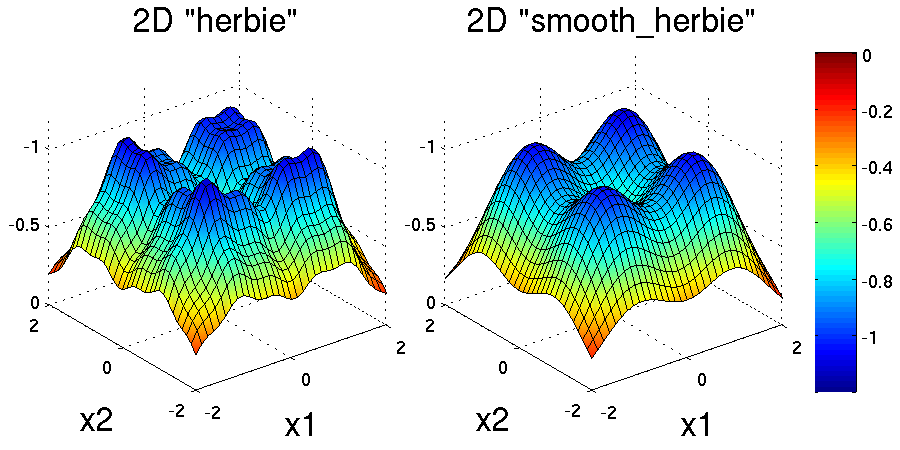
\includegraphics[scale=1.0]{images/DAK5pt2_2D__herbie__smooth_herbie}}
  \caption{Plots of the \texttt{herbie} (left) and
           \texttt{smooth\_herbie} (right) test functions in 2
           dimensions. They can accept an arbitrary number of
           inputs. The direction of the z-axis has been reversed 
           (negative is up) to better view the functions' minima.}
  \label{fig:2D_herbie__smooth_herbie}
\end{figure}

Shubert is another separable (and therefore arbitrary dimensional) 
test function. Its analytical formula is
\begin{displaymath}
{\rm shu}(\underline{x})=\prod_{k=1}^M w_{shu}\left(x_k\right)
\end{displaymath}
where 
\begin{displaymath}
w_{shu}\left(x_k\right)=\sum_{i=1}^5 i\cos((i+1)x_k+i)
\end{displaymath}
The 2D version of the \texttt{shubert} function is shown in 
Figure~\ref{fig:2D_shubert}. 

The DAKOTA input file \texttt{dakota\_separable\_ego\_5D.in} shows how
to use efficient global optimization (ego) to minimize the 5D version
of any of these 3 separable functions. Note that in the variables
section the \texttt{5*} preceding the values -2.0 and 2.0 for the
\texttt{lower\_bounds} and \texttt{upper\_bounds}, respectively, tells
DAKOTA to repeat them 5 times. The ``interesting'' region for each 
of these functions is $-2\le x_k \le 2$ for all dimensions.
\begin{center}
  \begin{small}
    \begin{bigbox}
      \verbatimtabinput[8]{dakota_separable_ego_5D.in}
    \end{bigbox}
  \end{small}
\end{center}

\begin{figure}
  \centering
  \centerline{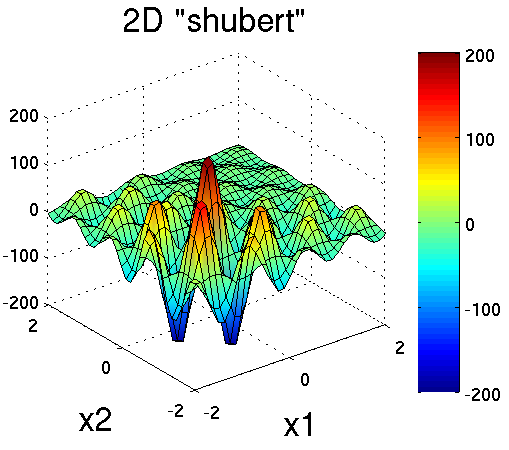
\includegraphics[scale=1.0]{images/DAK5pt2_2D_shubert}}
  \caption{Plot of the \texttt{shubert} test function in 2 dimensions.
           It can accept an arbitrary number of inputs.}
  \label{fig:2D_shubert}
\end{figure}

\section{Cylinder Head Example}\label{additional:cylinder}

The cylinder head example problem is stated as:
\begin{eqnarray}
\texttt{minimize }   & & f=-1\bigg(\frac{\mathtt{horsepower}}{250}+
  \frac{\mathtt{warranty}}{100000}\bigg) \nonumber\\
\texttt{subject to } & & \sigma_{max} \leq 0.5 \sigma_{yield}
  \label{additional:cylhead}\\
                     & & \mathtt{warranty} \geq 100000          \nonumber\\
                     & & \mathtt{time_{cycle}} \leq 60          \nonumber\\
                     & & 1.5 \leq \mathtt{d_{intake}} \leq 2.164\nonumber\\
                     & & 0.0 \leq \mathtt{flatness} \leq 4.0    \nonumber
\end{eqnarray}

This formulation seeks to simultaneously maximize normalized engine
horsepower and engine warranty over variables of valve intake diameter
($\mathtt{d_{intake}}$) in inches and overall head flatness
($\mathtt{flatness}$) in thousandths of an inch subject to inequality
constraints that the maximum stress cannot exceed half of yield, that
warranty must be at least 100000 miles, and that manufacturing cycle
time must be less than 60 seconds. Since the constraints involve
different scales, they should be nondimensionalized (note: the
nonlinear constraint scaling described in
Section~\ref{opt:additional:scaling} can now do this
automatically). In addition, they can be converted to the standard
1-sided form $g(\mathbf{x}) \leq 0$ as follows:
\begin{eqnarray}
  & & g_1=\frac{2\sigma_{\mathtt{max}}}{\sigma_{\mathtt{yield}}}-1 \leq 0
  \nonumber\\
  & & g_2=1-\frac{\mathtt{warranty}}{100000} \leq 0
  \label{additional:cylheadaltg}\\
  & & g_3=\frac{\mathtt{time_{cycle}}}{60}-1 \leq 0\nonumber
\end{eqnarray}

The objective function and constraints are related analytically to the
design variables according to the following simple expressions:
\begin{eqnarray}
\mathtt{warranty}     &=& 100000+15000(4-\mathtt{flatness})\nonumber\\
\mathtt{time_{cycle}} &=& 45+4.5(4-\mathtt{flatness})^{1.5}\nonumber\\
\mathtt{horsepower}   &=& 250+200\bigg(\frac{\mathtt{d_{intake}}}{1.833}-1\bigg)
  \label{additional:cylheadexp}\\
\sigma_{\mathtt{max}} &=& 750+\frac{1}{(\mathtt{t_{wall}})^{2.5}}\nonumber\\
\mathtt{t_{wall}}     &=& \mathtt{offset_{intake}-offset_{exhaust}}-
  \frac{(\mathtt{d_{intake}-d_{exhaust}})}{2}\nonumber
\end{eqnarray}

where the constants in Equation~\ref{additional:cylheadaltg} and
Equation~\ref{additional:cylheadexp} assume the following values:
$\sigma_{\mathtt{yield}}=3000$, $\mathtt{offset_{intake}}=3.25$,
$\mathtt{offset_{exhaust}}=1.34$, and $\mathtt{d_{exhaust}}=1.556$.

\subsection{Methods}\label{additional:cylinder:methods}

In the \texttt{Dakota/test} directory, the
\texttt{dakota\_cyl\_head.in} input file is used to execute a variety
of tests using the cylinder head example. One of these tests is shown
below and is available directly in \\ {\tt
Dakota/examples/methods/dakota\_addtnl\_cylhead.in}:
\begin{center}
  \begin{small}
    \begin{bigbox}
      \verbatimtabinput[8]{dakota_addtnl_cylhead.in}
    \end{bigbox}
  \end{small}
\end{center}

The interface keyword specifies use of the \texttt{cyl\_head}
executable (compiled from \texttt{Dakota/test/cyl\_head.C}) as the
simulator. The variables and responses keywords specify the data sets
to be used in the iteration by providing the initial point,
descriptors, and upper and lower bounds for two continuous design
variables and by specifying the use of one objective function, three
inequality constraints, and numerical gradients in the problem. The
method keyword specifies the use of the \texttt{npsol\_sqp} method to
solve this constrained optimization problem. No strategy keyword is
specified, so the default \texttt{single\_method} strategy is used.

\subsection{Optimization Results}\label{additional:cylinder:results}

The solution for the constrained optimization problem is:
\begin{eqnarray*}
    \mathrm{intake\_dia} &=& 2.122 \\
    \mathrm{flatness}    &=& 1.769
\end{eqnarray*}
with
\begin{eqnarray*}
      f^{\ast} &=& -2.461 \\
    g_1^{\ast} &=&  0.0    ~~\mathrm{(active)} \\
    g_2^{\ast} &=& -0.3347 ~~\mathrm{(inactive)} \\
    g_3^{\ast} &=&  0.0    ~~\mathrm{(active)}
\end{eqnarray*}
which corresponds to the following optimal response quantities:
\begin{eqnarray*}
    \mathrm{warranty}        &=& 133472 \\
    \mathrm{cycle\_time}     &=& 60 \\
    \mathrm{wall\_thickness} &=& 0.0707906 \\
    \mathrm{horse\_power}    &=& 281.579 \\
    \mathrm{max\_stress}     &=& 1500
\end{eqnarray*}

The final report from the DAKOTA output is as follows:
\begin{small}
\begin{verbatim}
    <<<<< Iterator npsol_sqp completed.					 
    <<<<< Function evaluation summary: 55 total (55 new, 0 duplicate)	 
    <<<<< Best parameters          =					 
                          2.1224188322e+00 intake_dia			 
                          1.7685568331e+00 flatness
    <<<<< Best objective function  =					 
                         -2.4610312954e+00
    <<<<< Best constraint values   =		 
                          1.8407497748e-13
                         -3.3471647504e-01
                          0.0000000000e+00
    <<<<< Best data captured at function evaluation 51
    <<<<< Single Method Strategy completed.
    DAKOTA execution time in seconds:					 
      Total CPU        =       0.04 [parent =   0.031995, child =   0.008005]
      Total wall clock =   0.232134
\end{verbatim}
\end{small}

\section{Container Example}\label{additional:container}

For this example, suppose that a high-volume manufacturer of light
weight steel containers wants to minimize the amount of raw sheet
material that must be used to manufacture a 1.1 quart
cylindrical-shaped can, including waste material. Material for the
container walls and end caps is stamped from stock sheet material of
constant thickness. The seal between the end caps and container wall
is manufactured by a press forming operation on the end caps. The end
caps can then be attached to the container wall forming a seal through
a crimping operation.
\begin{figure}
  \centering
  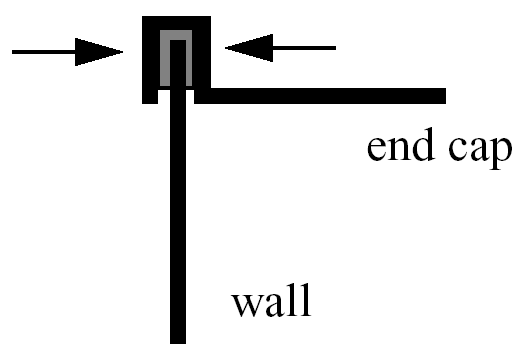
\includegraphics[scale=0.4]{images/end_cap}
  \caption{Container wall-to-end-cap seal}
  \label{additional:figure01}
\end{figure}

For preliminary design purposes, the extra material that would
normally go into the container end cap seals is approximated by
increasing the cut dimensions of the end cap diameters by 12\% and the
height of the container wall by 5\%, and waste associated with
stamping the end caps in a specialized pattern from sheet stock is
estimated as 15\% of the cap area. The equation for the area of the
container materials including waste is

\[
A=2 \times \left(\begin{array}{c}
    \mathtt{end\hbox{ }cap}\\
    \mathtt{waste}\\
    \mathtt{material}\\
    \mathtt{factor}
  \end{array} \right)
\times \left(\begin{array}{c}
    \mathtt{end\hbox{ }cap}\\
    \mathtt{seal}\\
    \mathtt{material}\\
    \mathtt{factor}
  \end{array} \right)
\times \left(\begin{array}{c}
    \mathtt{nominal}\\
    \mathtt{end\hbox{ }cap}\\
    \mathtt{area}
  \end{array} \right)
+ \left(\begin{array}{c}
    \mathtt{container}\\
    \mathtt{wall\hbox{ }seal}\\
    \mathtt{material}\\
    \mathtt{factor}
  \end{array} \right)
\times \left(\begin{array}{c}
    \mathtt{nominal}\\
    \mathtt{container}\\
    \mathtt{wall\hbox{ }area}
  \end{array} \right)
\]

or
\begin{equation}
A=2(1.15)(1.12)\pi\frac{D^2}{4}+(1.05)\pi DH \label{additional:contA}
\end{equation}

where $D$ and $H$ are the diameter and height of the finished product
in units of inches, respectively. The volume of the finished product
is specified to be
\begin{equation}
  V=\pi\frac{D^2H}{4}=(1.1\mathtt{qt})(57.75 \mathtt{in}^3/\mathtt{qt})
  \label{additional:contV}
\end{equation}

The equation for area is the objective function for this problem; it
is to be minimized. The equation for volume is an equality constraint;
it must be satisfied at the conclusion of the optimization problem.
Any combination of $D$ and $H$ that satisfies the volume constraint is
a \textbf{feasible} solution (although not necessarily the optimal
solution) to the area minimization problem, and any combination that
does not satisfy the volume constraint is an \textbf{infeasible}
solution. The area that is a minimum subject to the volume constraint
is the \textbf{optimal} area, and the corresponding values for the
parameters $D$ and $H$ are the optimal parameter values.

It is important that the equations supplied to a numerical
optimization code be limited to generating only physically realizable
values, since an optimizer will not have the capability to
differentiate between meaningful and nonphysical parameter values. It
is often up to the engineer to supply these limits, usually in the
form of parameter bound constraints. For example, by observing the
equations for the area objective function and the volume constraint,
it can be seen that by allowing the diameter, $D$, to become negative,
it is algebraically possible to generate relatively small values for
the area that also satisfy the volume constraint. Negative values for
$D$ are of course physically meaningless. Therefore, to ensure that
the numerically-solved optimization problem remains meaningful, a
bound constraint of $-D \leq 0$ must be included in the optimization
problem statement. A positive value for $H$ is implied since the
volume constraint could never be satisfied if $H$ were negative.
However, a bound constraint of $-H \leq 0$ can be added to the
optimization problem if desired. The optimization problem can then be
stated in a standardized form as
\begin{eqnarray}
\texttt{minimize}   & & 2(1.15)(1.12)\pi\frac{D^2}{4}+(1.05)^2\pi DH\nonumber\\
\texttt{subject to} & & \pi\frac{D^2H}{4}=
  (1.1\mathtt{qt})(57.75 \mathtt{in}^3/\mathtt{qt}) \label{additional:contFH}\\
                    & & -D \leq 0\hbox{, }-H \leq 0\nonumber
\end{eqnarray}

A graphical view of the container optimization problem appears in
Figure~\ref{additional:figure02}. The 3-D surface defines the area,
$A$, as a function of diameter and height. The curved line that
extends across the surface defines the areas that satisfy the volume
equality constraint, $V$. Graphically, the container optimization
problem can be viewed as one of finding the point along the constraint
line with the smallest 3-D surface height in
Figure~\ref{additional:figure02}. This point corresponds to the
optimal values for diameter and height of the final product.

\begin{figure}
  \centering
  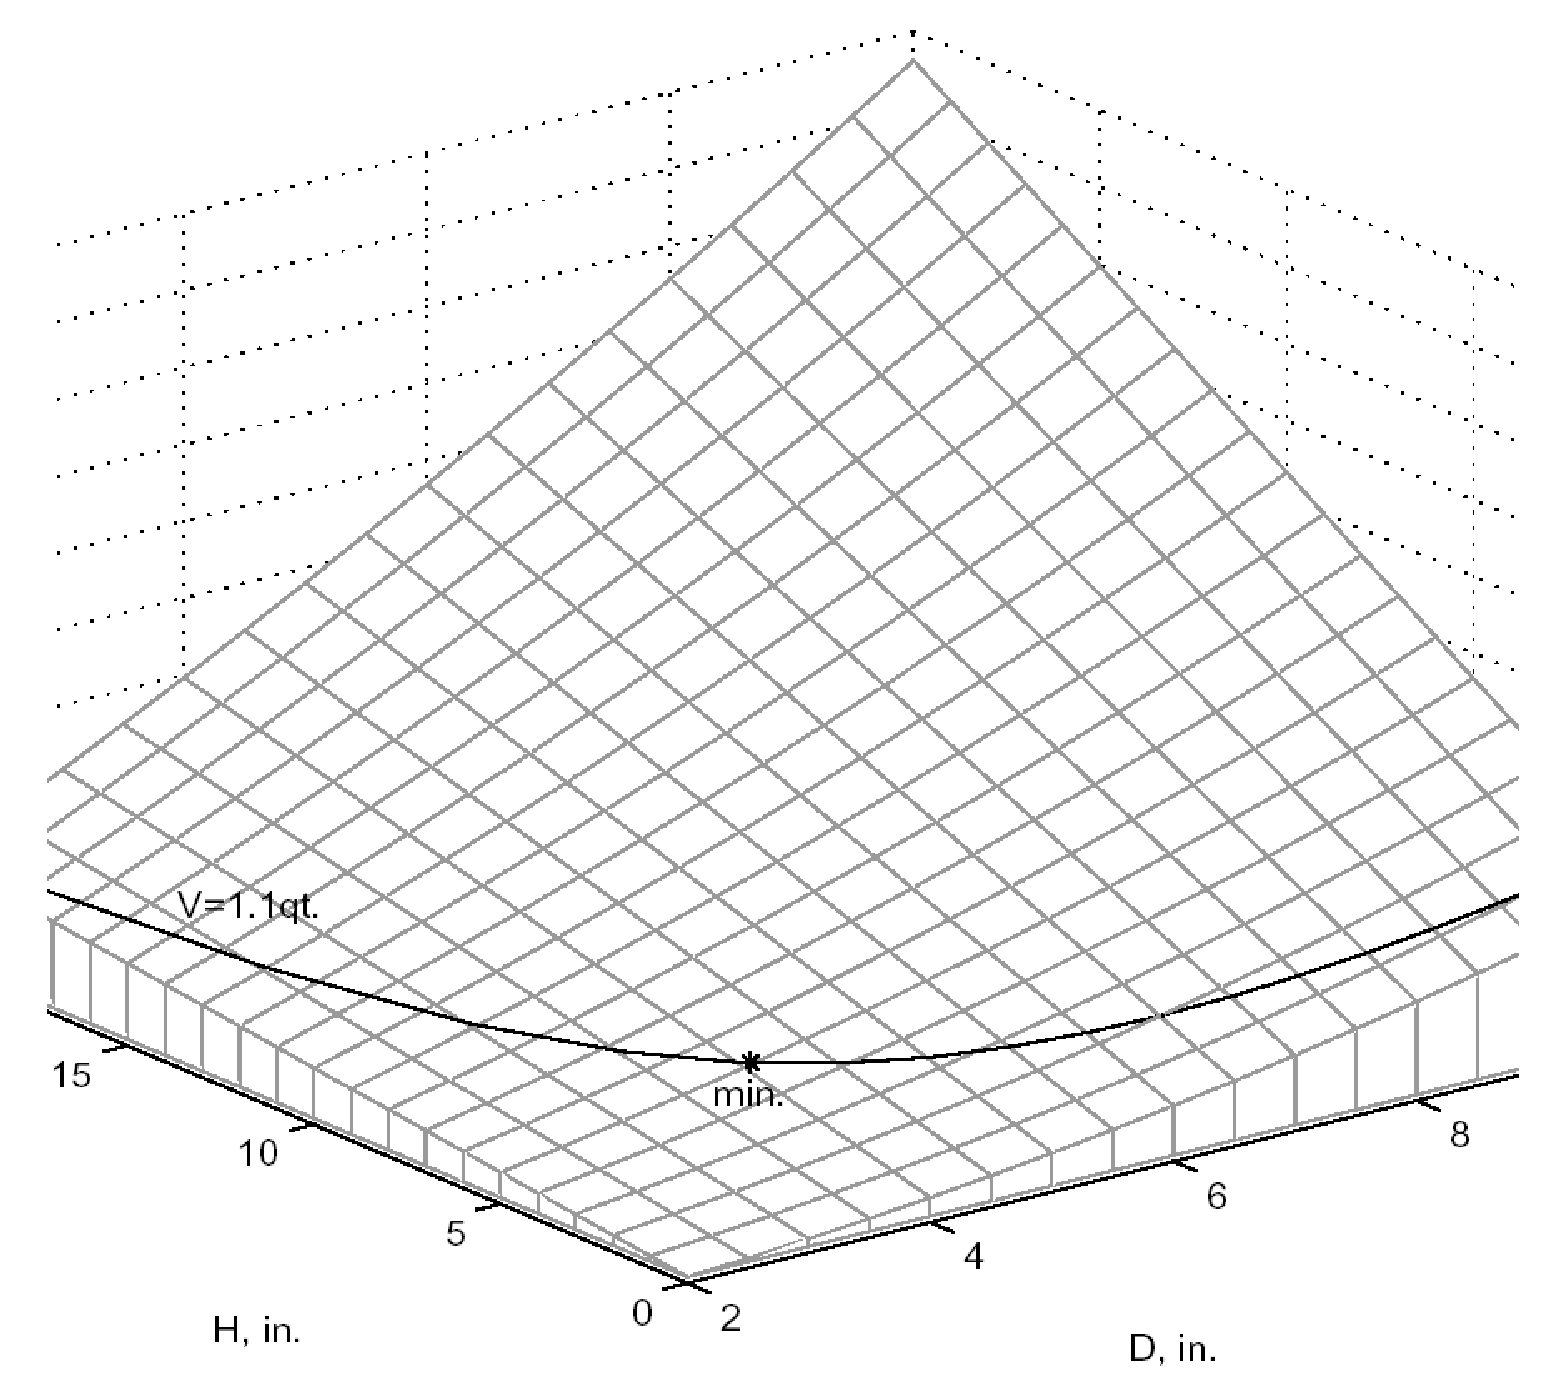
\includegraphics[scale=0.5]{images/graphical_container_opt}
  \caption{A graphical representation of the container optimization
    problem.}
  \label{additional:figure02}
\end{figure}

The input file for this test problem is named
\texttt{dakota\_container.in} in the directory \\
\texttt{Dakota/examples/methods}. The solution to this example
problem is $(H,D)=(4.99,4.03)$, with a minimum area of 98.43
$\mathtt{in}^2$ .

The final report from the DAKOTA output is as follows:
\begin{small}
\begin{verbatim}
    <<<<< Iterator npsol_sqp completed.
    <<<<< Function evaluation summary: 40 total (40 new, 0 duplicate)
    <<<<< Best parameters          =
                          4.9873894231e+00 H
                          4.0270846274e+00 D
    <<<<< Best objective function  =
                          9.8432498116e+01
    <<<<< Best constraint values   =
                         -9.6301439045e-12
    <<<<< Best data captured at function evaluation 36
    <<<<< Single Method Strategy completed.
    DAKOTA execution time in seconds:
      Total CPU        =      0.18 [parent =      0.18, child =         0]
      Total wall clock =  0.809126
\end{verbatim}
\end{small}

% Begin UQ testers

\section{Log Ratio Example}\label{additional:logratio}

This test problem, mentioned previously in
Section~\ref{uq:reliability:ex}, has a limit state function defined by
the ratio of two lognormally-distributed random variables.
\begin{equation}
g({\bf x}) = \frac{x_1}{x_2}
\end{equation}
The distributions for both $x_1$ and $x_2$ are Lognormal(1, 0.5) with
a correlation coefficient between the two variables of 0.3.

First-order and second-order reliability analysis are performed in the
\texttt{dakota\_logratio.in} and \\
\texttt{dakota\_logratio\_taylor2.in} input files in {\tt
Dakota/test}, respectively. For RIA, 24 response levels (.4, .5, .55,
.6, .65, .7, .75, .8, .85, .9, 1, 1.05, 1.15, 1.2, 1.25, 1.3, 1.35,
1.4, 1.5, 1.55, 1.6, 1.65, 1.7, and 1.75) are mapped into the
corresponding cumulative probability levels. For PMA, these 24
probability levels (the fully converged results from RIA FORM) are
mapped back into the original response levels.
Figure~\ref{fig:log_ratio_cdf} overlays the computed CDF values for a
number of first-order reliability method variants as well as a Latin
Hypercube reference solution of $10^6$ samples.
\begin{figure}
\centering
\centerline{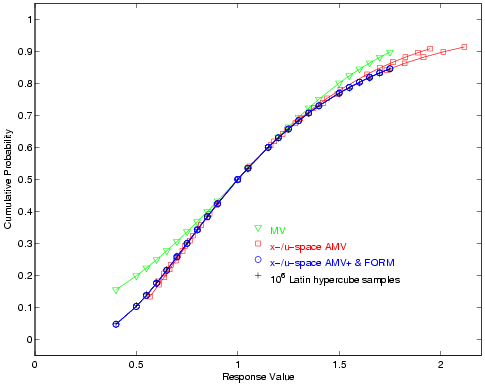
\includegraphics[scale=0.5]{images/log_ratio_cdf_ria}
            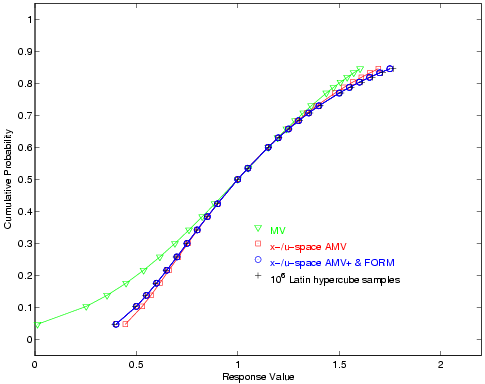
\includegraphics[scale=0.5]{images/log_ratio_cdf_pma}}
(a) RIA methods\hspace{2.5in}(b) PMA methods
\caption{Lognormal ratio cumulative distribution function, RIA/PMA methods.}
\label{fig:log_ratio_cdf}
\end{figure}

\section{Steel Section Example}\label{additional:steel_section}

This test problem is used extensively in~\cite{Hal00}. It involves a
W16x31 steel block of A36 steel that must carry an applied
deterministic bending moment of 1140 kip-in. For DAKOTA, it has been
used as a verification test for second-order integrations in
reliability methods. The limit state function is defined as:
\begin{equation}
g({\bf x}) = F_y Z - 1140
\end{equation}
where $F_y$ is Lognormal(38., 3.8), $Z$ is Normal(54., 2.7), and the
variables are uncorrelated.

The \texttt{Dakota/test/dakota\_steel\_section.in} input file computes
a first-order CDF probability of $p(g \leq 0.)$ = 1.297e-07 and a
second-order CDF probability of $p(g \leq 0.)$ = 1.375e-07. This
second-order result differs from that reported in~\cite{Hal00}, since
DAKOTA uses the Nataf nonlinear transformation to u-space (see MPP
Search Methods block in Reliability Methods chapter of DAKOTA Theory
Manual~\cite{TheoMan}) and \cite{Hal00} uses a linearized
transformation.

\section{Portal Frame Example}\label{additional:portal_frame}

This test problem is taken from~\cite{Tve90,Hon99}. It involves a
plastic collapse mechanism of a simple portal frame. It also has been
used as a verification test for second-order integrations in 
reliability methods. The limit state function is defined as:
\begin{equation}
g({\bf x}) = x_1 + 2 x_2 + 2 x_3 + x_4 - 5 x_5 - 5 x_6
\end{equation}
where $x_1 - x_4$ are Lognormal(120., 12.), $x_5$ is Lognormal(50.,
15.), $x_6$ is Lognormal(40., 12.), and the variables are uncorrelated.

While the limit state is linear in x-space, the nonlinear
transformation of lognormals to u-space induces curvature. The
\texttt{Dakota/test/dakota\_portal\_frame.in} input file computes a
first-order CDF probability of $p(g \leq 0.)$ = 9.433e-03 and a
second-order CDF probability of $p(g \leq 0.)$ = 1.201e-02. These
results agree with the published results from the literature.

% Begin UQ/OUU testers

\section{Short Column Example}\label{additional:short_column}

This test problem involves the plastic analysis and design of a short
column with rectangular cross section (width $b$ and depth $h$) having
uncertain material properties (yield stress $Y$) and subject to
uncertain loads (bending moment $M$ and axial force $P$)~\cite{Kus97}.
The limit state function is defined as:
\begin{equation}
g({\bf x}) = 1 - \frac{4M}{b h^2 Y} - \frac{P^2}{b^2 h^2 Y^2}
\end{equation}

The distributions for $P$, $M$, and $Y$ are Normal(500, 100),
Normal(2000, 400), and Lognormal(5, 0.5), respectively, with a
correlation coefficient of 0.5 between $P$ and $M$ (uncorrelated
otherwise). The nominal values for $b$ and $h$ are 5 and 15,
respectively.

\subsection{Uncertainty Quantification}

First-order and second-order reliability analysis are performed in the
\texttt{dakota\_short\_column.in} and \\
\texttt{dakota\_short\_column\_taylor2.in} input files in {\tt
Dakota/test}, respectively. For RIA, 43 response levels (-9.0, -8.75,
-8.5, -8.0, -7.75, -7.5, -7.25, -7.0, -6.5, -6.0, -5.5, -5.0, -4.5,
-4.0, -3.5, -3.0, -2.5, -2.0, -1.9, -1.8, -1.7, -1.6, -1.5, -1.4,
-1.3, -1.2, -1.1, -1.0, -0.9, -0.8, -0.7, -0.6, -0.5, -0.4, -0.3,
-0.2, -0.1, 0.0, 0.05, 0.1, 0.15, 0.2, 0.25) are mapped into the
corresponding cumulative probability levels. For PMA, these 43
probability levels (the fully converged results from RIA FORM) are
mapped back into the original response levels.
Figure~\ref{fig:short_col_cdf} overlays the computed CDF values for
several first-order reliability method variants as well as a Latin
Hypercube reference solution of $10^6$ samples.

\begin{figure}
\centering
\centerline{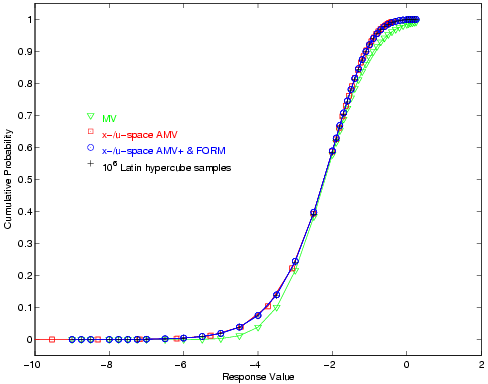
\includegraphics[scale=0.5]{images/short_col_cdf_ria}
            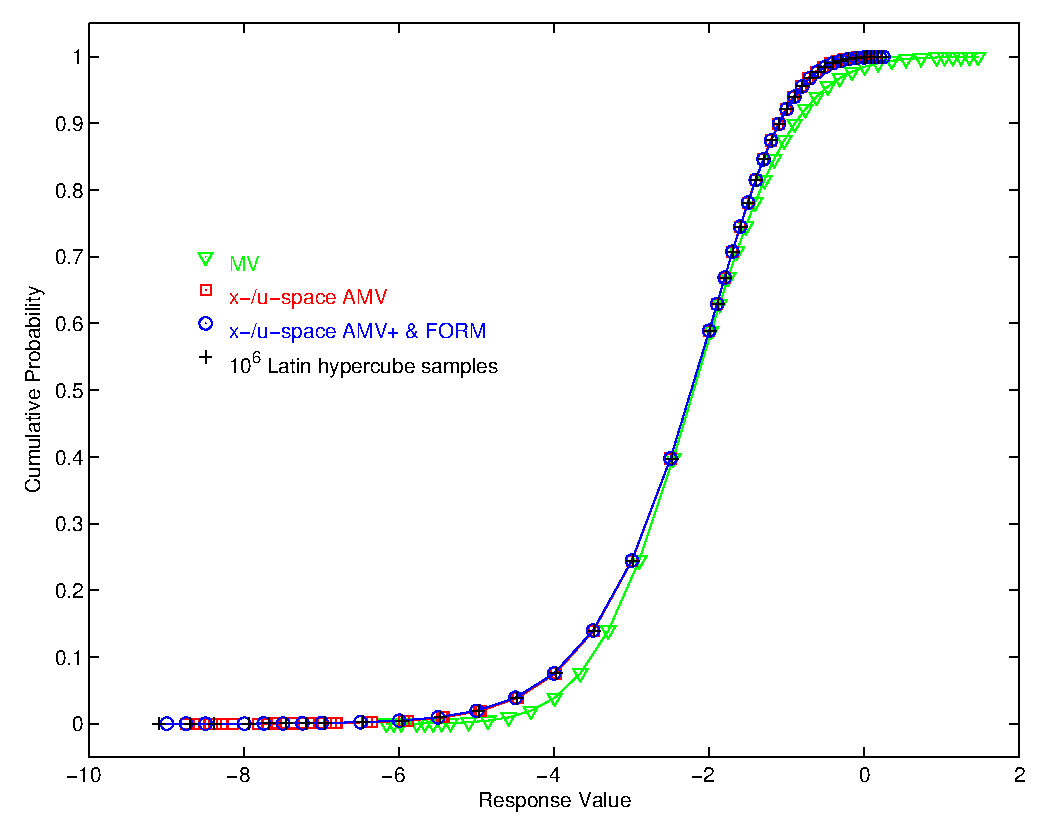
\includegraphics[scale=0.5]{images/short_col_cdf_pma}}
(a) RIA methods\hspace{2.75in}(b) PMA methods
\caption{Short column cumulative distribution function, RIA/PMA methods.}
\label{fig:short_col_cdf}
\end{figure}

\subsection{Reliability-Based Design Optimization}

The short column example problem is also amenable to RBDO. An
objective function of cross-sectional area and a target reliability
index of 2.5 (cumulative failure probability $p(g \le 0) \le 0.00621$) 
are used in the design problem:
\begin{eqnarray}
\min       & & bh \nonumber \\
{\rm s.t.} & & \beta \geq 2.5 \nonumber \\
           & &  5.0 \leq b \leq 15.0 \nonumber \\
           & & 15.0 \leq h \leq 25.0
\end{eqnarray}
As is evident from the UQ results shown in
Figure~\ref{fig:short_col_cdf}, the initial design of $(b, h) = (5,
15)$ is infeasible and the optimization must add material to obtain
the target reliability at the optimal design $(b, h) = (8.68, 25.0)$.
Simple bi-level, fully analytic bi-level, and sequential RBDO methods
are explored in {\tt Dakota/test} inputs \\
\texttt{dakota\_rbdo\_short\_column.in},
\texttt{dakota\_rbdo\_short\_column\_analytic.in}, and\\
\texttt{dakota\_rbdo\_short\_column\_trsb.in}, with results as
described in~\cite{Eld05,Eld06a}.

\section{Cantilever Example}\label{additional:cantilever}

This test problem is adapted from the reliability-based design
optimization literature~\cite{Sue01},~\cite{Wu01} and involves a simple
uniform cantilever beam as shown in Figure~\ref{additional:figure03}.

\begin{figure}
  \centering
  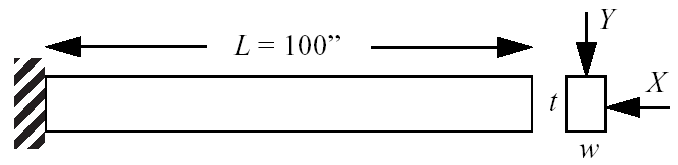
\includegraphics[scale=0.5]{images/cantilever_beam}
  \caption{Cantilever beam test problem.}
  \label{additional:figure03}
\end{figure}

The design problem is to minimize the weight (or, equivalently, the
cross-sectional area) of the beam subject to a displacement constraint
and a stress constraint. Random variables in the problem include the
yield stress $R$ of the beam material, the Young's modulus $E$ of the
material, and the horizontal and vertical loads, $X$ and $Y$, which
are modeled with normal distributions using $N(40000, 2000)$,
$N(2.9E7, 1.45E6)$, $N(500, 100)$, and $N(1000, 100)$, respectively.
Problem constants include $L = 100\mathtt{in}$ and $D_{0} = 2.2535
\mathtt{in}$. The constraints have the following analytic form:
\begin{eqnarray}
\mathtt{stress}&=&\frac{600}{w t^2}Y+\frac{600}{w^2t}X \leq R
  \label{additional:cant}\\
\mathtt{displacement}&=&\frac{4L^3}{E w t}
  \sqrt{\bigg(\frac{Y}{t^2}\bigg)^2+\bigg(\frac{X}{w^2}\bigg)^2}
  \leq D_{0} \nonumber
\end{eqnarray}
or when scaled:
\begin{eqnarray}
  g_{S}&=&\frac{\mathtt{stress}}{R}-1 \leq 0\label{additional:cantscale}\\
  g_{D}&=&\frac{\mathtt{displacement}}{D_{0}}-1 \leq 0\nonumber\\
\end{eqnarray}

\subsection{Deterministic Optimization Results}\label{additional:cantilever:deterministic}

If the random variables $E$, $R$, $X$, and $Y$ are fixed at their
means, the resulting deterministic design problem can be formulated as
\begin{eqnarray}
\texttt{minimize }   & & f = w t            \nonumber\\
\texttt{subject to } & & g_{S} \leq 0 \label{additional:cantopt}\\
                     & & g_{D} \leq 0       \nonumber\\
                     & & 1.0 \leq w \leq 4.0\nonumber\\
                     & & 1.0 \leq t \leq 4.0\nonumber
\end{eqnarray}
and can be solved using the \texttt{Dakota/test/dakota\_cantilever.in}
file. This input file manages a variety of tests, of which a sample is
shown below \\
(\texttt{Dakota/examples/methods/dakota\_addtnl\_cantilever.in}):
\begin{center}
  \begin{small}
    \begin{bigbox}
      \verbatimtabinput[8]{dakota_addtnl_cantilever.in}
    \end{bigbox}
  \end{small}
\end{center}

The deterministic solution is $(w,t)=(2.35,3.33)$ with an objective
function of $7.82$. The final report from the DAKOTA output is as
follows:
\begin{small}
\begin{verbatim}
    <<<<< Iterator npsol_sqp completed.
    <<<<< Function evaluation summary: 33 total (33 new, 0 duplicate)
    <<<<< Best parameters          =
                          2.3520341271e+00 beam_width
                          3.3262784077e+00 beam_thickness
                          4.0000000000e+04 R
                          2.9000000000e+07 E
                          5.0000000000e+02 X
                          1.0000000000e+03 Y
    <<<<< Best objective function  =
                          7.8235203313e+00
    <<<<< Best constraint values   =
                         -1.6009000260e-02
                         -3.7083558446e-11
    <<<<< Best data captured at function evaluation 31
    <<<<< Single Method Strategy completed.
    DAKOTA execution time in seconds:
      Total CPU        =       0.03 [parent =   0.027995, child =   0.002005]
      Total wall clock =   0.281375
\end{verbatim}
\end{small}

\subsection{Stochastic Optimization Results}\label{additional:cantilever:stochastic}

If the normal distributions for the random variables $E$, $R$, $X$,
and $Y$ are included, a stochastic design problem can be formulated as
\begin{eqnarray}
\texttt{minimize }   & & f = w t            \nonumber\\
\texttt{subject to } & & \beta_{D} \geq 3   \label{additional:cantouu}\\
                     & & \beta_{S} \geq 3   \nonumber\\
                     & & 1.0 \leq w \leq 4.0\nonumber\\
                     & & 1.0 \leq t \leq 4.0\nonumber
\end{eqnarray}
where a 3-sigma reliability level (probability of failure = 0.00135 if
responses are normally-distributed) is being sought on the scaled
constraints. Optimization under uncertainty solutions to the
stochastic problem are described in~\cite{Eld02,Eld05,Eld06a}, for
which the solution is $(w,t)=(2.45,3.88)$ with an objective function
of $9.52$. This demonstrates that a more conservative design is
needed to satisfy the probabilistic constraints.

\subsection{Interval Analysis}\label{tutorial:example:uncert_quant:interval}

Interval analysis is often used to model epistemic uncertainty. 
In interval analysis, one assumes that nothing is known about 
an epistemic uncertain variable except that its value lies 
somewhere within an interval. In this situation, it is NOT 
assumed that the value has a uniform probability of occuring 
within the interval. Instead, the interpretation is that 
any value within the interval is a possible value or a potential 
realization of that variable. In interval analysis, the 
uncertainty quantification problem is one of determining the 
resulting bounds on the output (defining the output interval) 
given interval bounds on the inputs. Again, any output response 
that falls within the output interval is a possible output 
with no frequency information assigned to it.

We can do interval analysis using either
\texttt{global\_interval\_est} or \texttt{local\_interval\_est}.
In the global approach, one uses either a global optimization 
method or a sampling method to assess the bounds, whereas the 
local method uses gradient information in a derivative-based 
optimization approach. 
 
An example of interval estimation 
is found in the test file \texttt{dakota\_uq\_interval.in}, 
and also in Figure~\ref{additional:interval}, with example results in 
Figure~\ref{additional:interval_out}. This example is a demonstration 
of calculating interval bounds for three outputs of the cantilever beam 
problem. The cantilever beam problem is described in detail in 
Section~\ref{additional:cantilever}. Given input intervals of [1,10] on 
beam width and beam thickness, we can see that the interval estimate of 
beam weight is approximately [1,100].

\begin{figure}
  \centering
  \begin{bigbox}
    \begin{small}
      \verbatimtabinput[8]{dakota_uq_interval.in}
    \end{small}
  \end{bigbox}
\caption{DAKOTA input file for performing UQ using interval analysis.}
\label{additional:interval}
\end{figure}

\begin{figure}
\centering
\begin{bigbox}
\begin{small}
\begin{verbatim}
------------------------------------------------------------------
Min and Max estimated values for each response function:
weight:  Min = 1.0000169352e+00  Max = 9.9999491948e+01
stress:  Min = -9.7749994284e-01  Max = 2.1499428450e+01
displ:  Min = -9.9315672724e-01  Max = 6.7429714485e+01
-----------------------------------------------------------------
\end{verbatim}
\end{small}
\end{bigbox}
\caption{Excerpt of UQ output for interval example.}
\label{additional:interval_out}
\end{figure}

\section{Steel Column Example}\label{additional:steel_column}

This test problem involves the trade-off between cost and
reliability for a steel column~\cite{Kus97}. The cost is defined as
\begin{equation}
Cost = b d + 5 h
\end{equation}
where $b$, $d$, and $h$ are the means of the flange breadth, flange
thickness, and profile height, respectively. Nine uncorrelated random
variables are used in the problem to define the yield stress $F_s$
(lognormal with $\mu/\sigma$ = 400/35 MPa), dead weight load $P_1$
(normal with $\mu/\sigma$ = 500000/50000 N), variable load $P_2$
(gumbel with $\mu/\sigma$ = 600000/90000 N), variable load $P_3$
(gumbel with $\mu/\sigma$ = 600000/90000 N), flange breadth $B$
(lognormal with $\mu/\sigma$ = $b$/3 mm), flange thickness $D$
(lognormal with $\mu/\sigma$ = $d$/2 mm), profile height $H$
(lognormal with $\mu/\sigma$ = $h$/5 mm), initial deflection $F_0$
(normal with $\mu/\sigma$ = 30/10 mm), and Young's modulus $E$ (Weibull
with $\mu/\sigma$ = 21000/4200 MPa). The limit state has the
following analytic form:
\begin{equation}
g = F_s - P \left( \frac{1}{2 B D} + 
\frac{F_0}{B D H} \frac{E_b}{E_b - P} \right)\\
\end{equation}
where
\begin{eqnarray}
P   & = & P_1 + P_2 + P_3 \\
E_b & = & \frac{\pi^2 E B D H^2}{2 L^2}
\end{eqnarray}
and the column length $L$ is 7500 mm.

This design problem (\texttt{dakota\_rbdo\_steel\_column.in} in
\texttt{Dakota/test}) demonstrates design variable insertion into
random variable distribution parameters through the design of the mean
flange breadth, flange thickness, and profile height. The RBDO
formulation maximizes the reliability subject to a cost constraint:
\begin{eqnarray}
{\rm maximize }   & & \beta                   \nonumber \\
{\rm subject to } & & Cost  \leq 4000.       \nonumber \\
                  & & 200.0 \leq b \leq 400.0 \\
                  & &  10.0 \leq d \leq  30.0 \nonumber \\
                  & & 100.0 \leq h \leq 500.0 \nonumber
\end{eqnarray}
which has the solution ($b$, $d$, $h$) = (200.0, 17.50, 100.0) with a
maximal reliability of 3.132.

\section{Multiobjective Examples}\label{additional:multiobjective}

Multiobjective optimization means that there are two or more
objective functions that you wish to optimize simultaneously. Often
these are conflicting objectives, such as cost and performance. The
answer to a multi-objective problem is usually not a single point.
Rather, it is a set of points called the Pareto front. Each point
on the Pareto front satisfies the Pareto optimality criterion, i.e.,
locally there exists no other feasible vector that would improve some
objective without causing a simultaneous worsening in at least one
other objective. Thus a feasible point $X^\prime$ from which
small moves improve one or more objectives without worsening
any others is not Pareto optimal: it is said to be ``dominated''
and the points along the Pareto front are said to be
``non-dominated''.

Often multi-objective problems are addressed by simply assigning
weights to the individual objectives, summing the weighted
objectives, and turning the problem into a single-objective one
which can be solved with a variety of optimization techniques. While
this approach provides a useful ``first cut'' analysis (and is
supported within DAKOTA---see Section~\ref{opt:additional}), this
approach has many limitations. The major limitation is that a
local solver with a weighted sum objective will only find one
% optimal solutions if the true Pareto front is nonconvex. %Hogwash!
point on the Pareto front; if one wants to understand
the effects of changing weights, this method can be computationally
expensive. Since each optimization of a single weighted objective
will find only one point on the Pareto front, many
optimizations must be performed to get a good parametric
understanding of the influence of the weights and to achieve a good
sampling of the entire Pareto frontier.

Starting with version 3.2 of DAKOTA, a capability to perform
multi-objective optimization based on a genetic algorithm method has
been available. This method is called \texttt{moga}. It is based on
the idea that as the population evolves in a GA, solutions that are
non-dominated are chosen to remain in the population. Until version
4.0 of DAKOTA, there was a selection\_type choice of domination\_count
that performed a custom fitness assessment and selection operation
together. As of version 4.0 of DAKOTA, that functionality has been
broken into separate, more generally usable fitness assessment and
selection operators called the domination\_count fitness assessor and
below\_limit selector respectively. The effect of using these two
operators is the same as the previous behavior of the
domination\_count selector. This means of selection works especially
well on multi-objective problems because it has been specifically
designed to avoid problems with aggregating and scaling objective
function values and transforming them into a single
objective. Instead, the fitness assessor works by ranking population
members such that their resulting fitness is a function of the number
of other designs that dominate them. The below\_limit selector then
chooses designs by considering the fitness of each. If the fitness of
a design is above a certain limit, which in this case corresponds to a
design being dominated by more than a specified number of other
designs, then it is discarded. Otherwise it is kept and selected to go
to the next generation. The one catch is that this selector will
require that a minimum number of selections take
place. The \texttt{shrinkage\_percentage} determines the minimum number of
selections that will take place if enough designs are available. It is
interpreted as a percentage of the population size that must go on to
the subsequent generation. To enforce this, the below\_limit selector
makes all the selections it would make anyway and if that is not
enough, it relaxes its limit and makes selections from the remaining
designs. It continues to do this until it has made enough selections.
The moga method has many other important features. Complete
descriptions can be found in the DAKOTA Reference Manual~\cite{RefMan}.


There are three examples %in the test directory ({\tt
%Dakota/test/dakota\_mogatest.in}) 
that are taken from a multiobjective %there are no examples in test dir. they are in tutorial and methods, but should all be moved to methods
evolutionary algorithm (MOEA) test suite described by Van Veldhuizen
et. al. in~\cite{Coe02}. These three examples 
illustrate the different forms that the Pareto set may take. For each
problem, we describe the DAKOTA input and show a graph of the Pareto
front. These problems are all solved with the \texttt{moga} method.
In Van Veldhuizen's notation, the set of all Pareto optimal design
configurations (design variable values only) is denoted $\mathtt{P^*}$
or $\mathtt{P_{true}}$ and is defined as:
\begin{eqnarray*}
  P^*:=\{x\in\Omega\,|\,\neg\exists\,\,
  x^\prime\in\Omega\quad\bar{f}(x^\prime)\preceq\bar{f}(x)\}
\end{eqnarray*}

The Pareto front, which is the set of objective function values
associated with the Pareto optimal design configurations, is denoted
$\mathtt{PF^*}$ or $\mathtt{PF_{true}}$ and is defined as:
\begin{eqnarray*}
  PF^*:=\{\bar{u}=\bar{f}=(f_1(x),\ldots,f_k(x))\,|\, x\in P^*\}
\end{eqnarray*}

The values calculated for the Pareto set and the Pareto front using
the moga method are close to but not always exactly the true values,
depending on the number of generations the moga is run, the various
settings governing the GA, and the complexity of the Pareto set.

Sections~\ref{opt:software} and~\ref{opt:additional} provide more
information on multiobjective optimization.


\subsection{Multiobjective Test Problem 1}\label{additional:multiobjective:problem1}

The first test problem is a case where $P_{true}$ is connected and
$PF_{true}$ is concave. The problem is to simultaneously optimize
$f_1$ and $f_2$ given three input variables, $x_1$, $x_2$, and
$x_3$, where the inputs are bounded by $-4 \leq x_{i} \leq 4$:

Figure~\ref{additional:moga1inp} shows an input file that
demonstrates some of the multi-objective capabilities available with
the moga method.
\begin{figure}[htp!]
  \centering
  \begin{bigbox}
    \begin{small}
      \verbatimtabinput[8]{dakota_mogatest1.in}
    \end{small}
  \end{bigbox}
  \caption{Multiple objective genetic algorithm (MOGA) example: the
    DAKOTA input file.}
  \label{additional:moga1inp}
\end{figure}

%This example has three input variables and two objectives.
% The example uses objectives different from the Rosenbrock
% function because we wanted to demonstrate the capability on a problem
% with two conflicting objectives. 
%This example is taken from a testbed
%of multi-objective problems~\cite{Coe02}. 
In this example, the three best 
solutions (as specified by \texttt{final\_solutions} =3) are written to the 
output. Additionally, final results from moga
are output to a file called \texttt{finaldata1.dat} in the directory in
which you are running. This \texttt{finaldata1.dat} file is simply a
list of inputs and outputs. Plotting the output columns against each
other allows one to see the Pareto front generated by \texttt{moga}.
Figure~\ref{additional:moga_pareto} shows an example of the Pareto
front for this problem. Note that a Pareto front easily shows the
tradeoffs between Pareto optimal solutions. For example, look at the
point with f1 and f2 values equal to (0.9, 0.23). One cannot improve
(minimize) the value of objective function f1 without increasing the
value of f2: another point on the Pareto front, (0.63, 0.63) represents
a better value of objective f1 but a worse value of objective f2.
\begin{figure}[ht!]
  \centering
  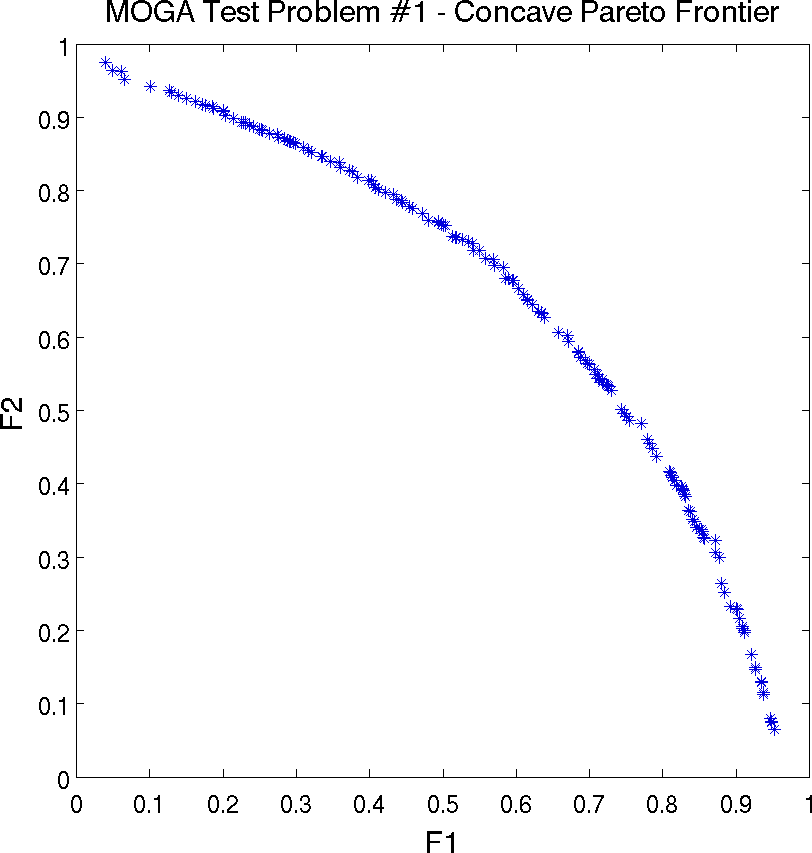
\includegraphics[scale=0.75]{images/dakota_mogatest1_pareto_front}
  \caption{Multiple objective genetic algorithm (MOGA) example: Pareto
  front showing tradeoffs between functions f1 and f2.}
  \label{additional:moga_pareto}
\end{figure}

\subsection{Multiobjective Test Problem 2}\label{additional:multiobjective:problem2}

The second test problem is a case where both $\mathtt{P_{true}}$ and
$\mathtt{PF_{true}}$ are disconnected. $\mathtt{PF_{true}}$ has four
separate Pareto curves. The problem is to simultaneously optimize
$f_1$ and $f_2$ given two input variables, $x_1$ and $x_2$,
where the inputs are bounded by $0 \leq x_{i} \leq 1$, and:
\begin{eqnarray*}
f_1(x) &=& x_1 \\
f_2(x) &=& (1+10x_2) \times \left[1-\bigg(\frac{x_1}{1+10x_2}\bigg)^2-
\frac{x_1}{1+10x_2}\sin(8\pi x_1)\right]
\end{eqnarray*}

The input file for this example is shown in
Figure~\ref{additional:moga2inp} and provided in \\ {\tt
Dakota/examples/methods/dakota\_mogatest2.in} . It differs from
Figure~\ref{additional:moga1inp} in the variables specification, in
the use of the \texttt{mogatest2} executable (compiled from
\texttt{Dakota/test/mogatest2.C}) as the simulator, and in the
\texttt{max\_function\_evaluations} and \texttt{crossover\_type} MOGA
controls. The Pareto front is shown in
Figure~\ref{additional:moga2front}. Note the discontinuous nature of
the front in this example.

\begin{figure}
  \centering
  \begin{bigbox}
    \begin{small}
      \verbatimtabinput[8]{dakota_mogatest2.in}
    \end{small}
  \end{bigbox}
  \caption{DAKOTA input file specifying the use of MOGA on mogatest2}
  \label{additional:moga2inp}
\end{figure}

\begin{figure}
  \centering
  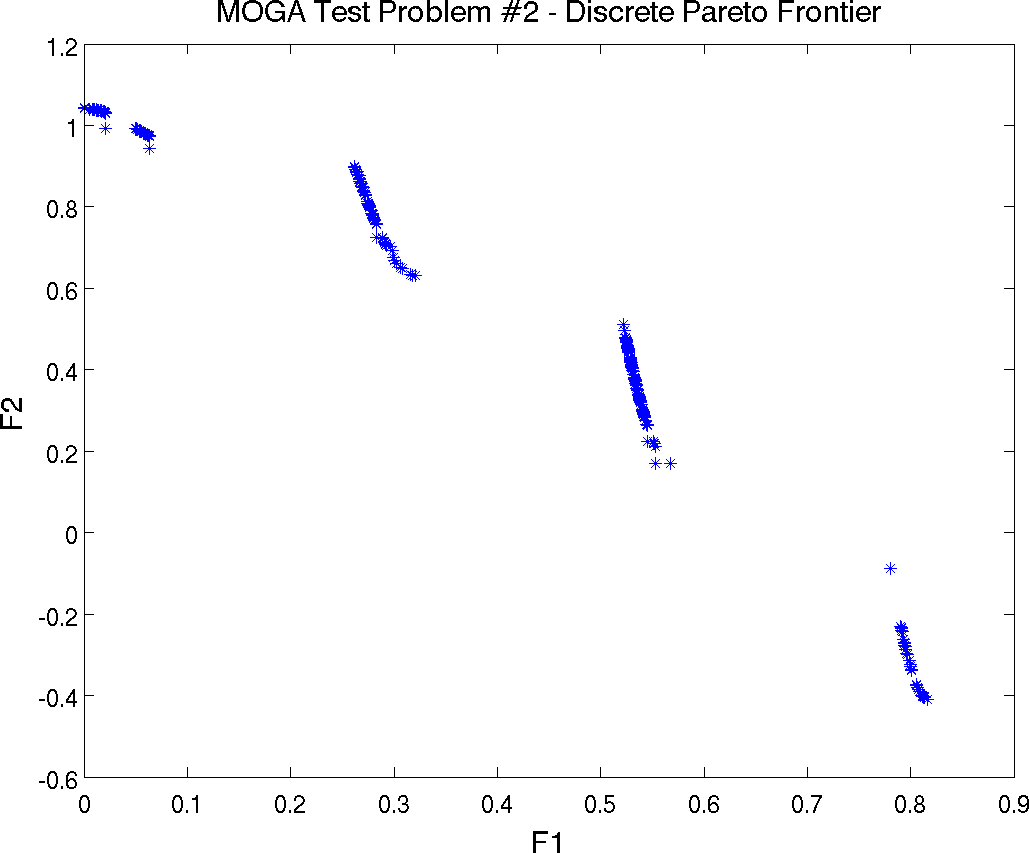
\includegraphics[scale=0.75]{images/dakota_mogatest2_pareto_front}
  \caption{Pareto Front showing Tradeoffs between Function F1 and
    Function F2 for mogatest2}
  \label{additional:moga2front}
\end{figure}

\subsection{Multiobjective Test Problem 3}\label{additional:multiobjective:problem3}

The third test problem is a case where $\mathtt{P_{true}}$ is
disconnected but $\mathtt{PF_{true}}$ is connected. It is called the
Srinivas problem in the literature (cite). This problem also has two
nonlinear constraints. The problem is to simultaneously optimize
$f_1$ and $f_2$ given two input variables, $x_1$ and $x_2$,
where the inputs are bounded by $-20 \leq x_{i} \leq 20$, and:
\begin{eqnarray*}
f_1(x) &=& (x_1-2)^2+(x_2-1)^2+2 \\
f_2(x) &=& 9x_1-(x_2-1)^2
\end{eqnarray*}

The constraints are:
\begin{eqnarray*}
0 &\leq& x_1^2+x_2^2-225 \\
0 &\leq& x_1-3x_2+10
\end{eqnarray*}

The input file for this example is shown in
Figure~\ref{additional:moga3inp} and provided in \\ {\tt
Dakota/examples/methods/dakota\_mogatest3.in}. It differs from
Figure~\ref{additional:moga2inp} in the variables and responses
specifications, in the use of the \texttt{mogatest3} executable
(compiled from \texttt{Dakota/test/mogatest3.C}) as the simulator, and
in the \texttt{max\_function\_evaluations} and \texttt{mutation\_type}
MOGA controls. The Pareto set is shown in
Figure~\ref{additional:moga3set}. Note the discontinuous nature of the
Pareto set (in the design space) in this example. The Pareto front is
shown in Figure~\ref{additional:moga3front}.
%Again, note the unusual nature of this Pareto example (these figures 
%agree reasonably well with the Srinivas problem results shown in the 
%literature).

\begin{figure}
  \centering
  \begin{bigbox}
    \begin{small}
      \verbatimtabinput[8]{dakota_mogatest3.in}
    \end{small}
  \end{bigbox}
  \caption{DAKOTA input file specifying the use of MOGA on mogatest3}
  \label{additional:moga3inp}
\end{figure}

\begin{figure}
  \centering
  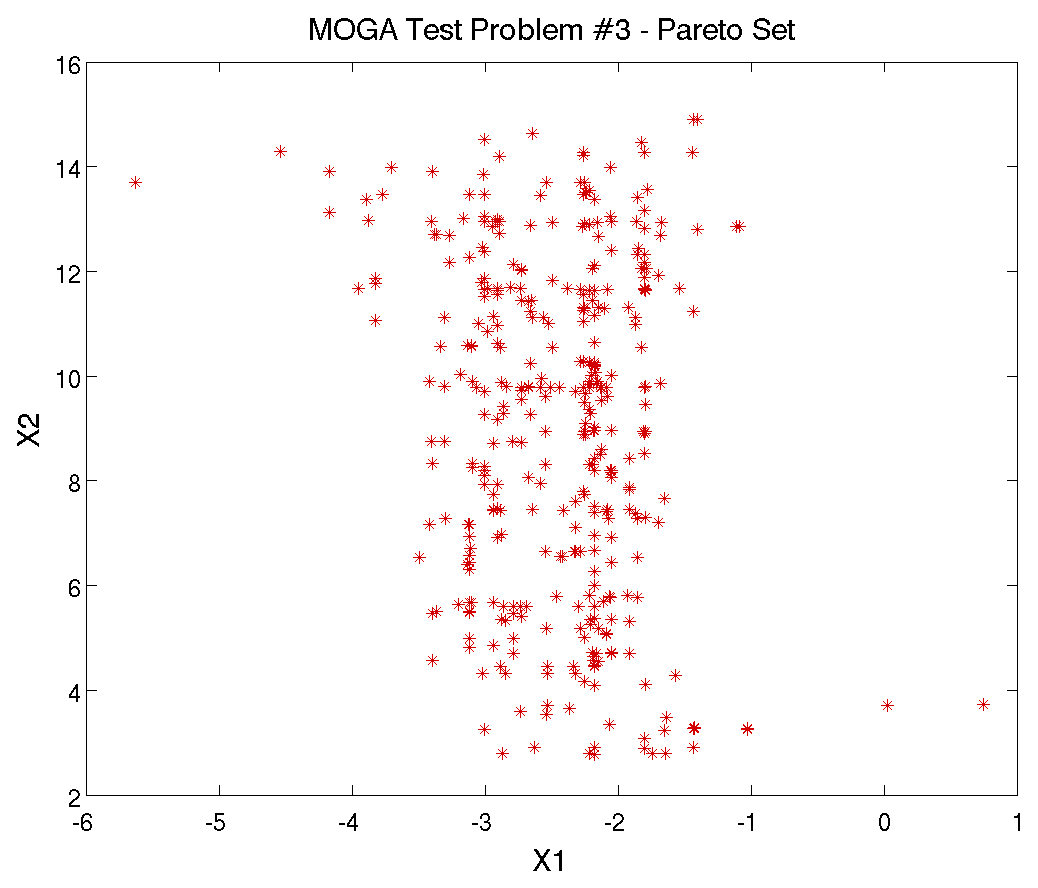
\includegraphics[scale=0.75]{images/dakota_mogatest3_pareto_set}
  \caption{Pareto Set of Design Variables corresponding to the Pareto
    front for mogatest3}
  \label{additional:moga3set}
\end{figure}

\begin{figure}
  \centering
  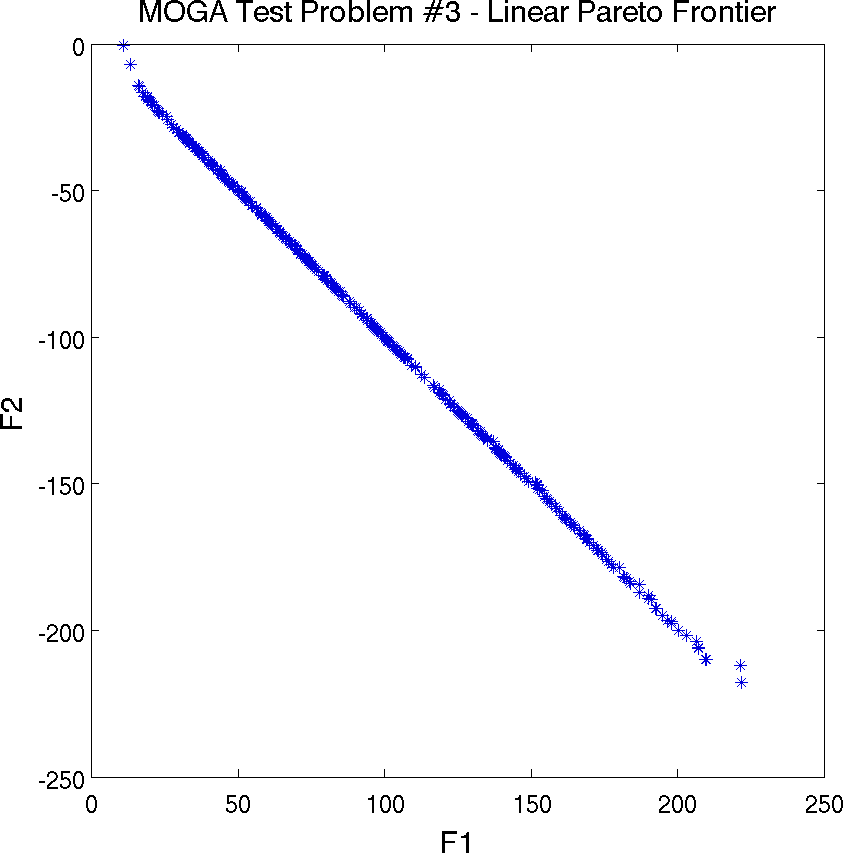
\includegraphics[scale=0.75]{images/dakota_mogatest3_pareto_front}
  \caption{Pareto Front showing Tradeoffs between Function F1 and
    Function F2 for mogatest3}
  \label{additional:moga3front}
\end{figure}

\section{Morris example}\label{additional:morris}

Morris~\cite{Mor91} includes a screening design test problem with a
single-output analytical test function. The output depends on 20
inputs with first- through fourth-order interaction terms, some having
large fixed coefficients and others small random coefficients. Thus
the function values generated depend on the random number generator
employed in the function evaluator. The computational model is:

\begin{align*}
y = &\;\beta_0 + \sum_{i=1}^{20}{\beta_i w_i} + \sum_{i<j}^{20}{\beta_{i,j} w_i w_j} + \sum_{i<j<l}^{20}{\beta_{i,j,l} w_i w_j w_l} \\
    &+  \sum_{i<j<l<s}^{20}{\beta_{i,j,l,s} w_i w_j w_l w_s},
\end{align*}
where $w_i = 2(x_i-0.5)$ except for $i=3, 5, \mbox{ and } 7$, where $w_i=2(1.1x_i/(x_i+0.1) - 0.5)$. Large-valued coefficients are assigned as 
\begin{align*}
&\beta_i = +20 & &i=1,\ldots,10; \;&\beta_{i,j} = -15& &i,j = 1, \ldots, 6; \\
&\beta_{i,j,l} = -10& &i,j,l=1,\ldots,5; \;&\beta_{i,j,l,s} = +5& &i,j,l,s = 1, \ldots, 4.
\end{align*}
The remaining first- and second-order coefficients $\beta_i$ and
$\beta_{i,j}$, respectively, are independently generated from a
standard normal distribution (zero mean and unit standard deviation);
the remaining third- and fourth-order coefficients are set to zero.

Examination of the test function reveals that one should be able to
conclude the following (stated and verified computationally
in~\cite{Sal04}) for this test problem:
\begin{enumerate}
\item the first ten factors are important;
\item of these, the first seven have significant effects involving
      either interactions or curvatures; and
\item the other three are important mainly because of their first-order
      effect.
\end{enumerate}

The dakota test input {\tt Dakota/test/dakota\_psuade.in} exercises
the MOAT algorithm described in Section~\ref{dace:psuade} on the
Morris problem. The DAKOTA output obtained is shown in
Figures~\ref{FIG:moat:out_preamble} and~\ref{FIG:moat:out_results}.
\begin{figure}[ht!]
\centering
\begin{bigbox}
\begin{small}
\begin{verbatim}
Running MPI executable in serial mode.
DAKOTA version 5.0+ developmental release.
Subversion revision 172 built Dec  8 2010 17:35:13.
Constructing Single Method Strategy...
Writing new restart file dakota.rst
methodName = psuade_moat
gradientType = none
hessianType = none

>>>>> Running Single Method Strategy.

>>>>> Running psuade_moat iterator.

PSUADE DACE method = psuade_moat Samples = 84 Seed (user-specified) = 500
            Partitions = 3 (Levels = 4)
\end{verbatim}
\end{small}
\end{bigbox}
\caption[DAKOTA initialization output for PSUADE
MOAT.]{\label{FIG:moat:out_preamble} DAKOTA initialization output for
the PSUADE MOAT method on the Morris test problem showing the study
parameters.}
\end{figure}
\begin{figure}[ht!]
\centering
\begin{bigbox}
\begin{small}
\begin{verbatim}
>>>>>> PSUADE MOAT output for function 0:

*************************************************************
*********************** MOAT Analysis ***********************
-------------------------------------------------------------
Input   1 (mod. mean & std) =   9.5329e+01   9.0823e+01 
Input   2 (mod. mean & std) =   6.7297e+01   9.5242e+01 
Input   3 (mod. mean & std) =   1.0648e+02   1.5479e+02 
Input   4 (mod. mean & std) =   6.6231e+01   7.5895e+01 
Input   5 (mod. mean & std) =   9.5717e+01   1.2733e+02 
Input   6 (mod. mean & std) =   8.0394e+01   9.9959e+01 
Input   7 (mod. mean & std) =   3.2722e+01   2.7947e+01 
Input   8 (mod. mean & std) =   4.2013e+01   7.6090e+00 
Input   9 (mod. mean & std) =   4.1965e+01   7.8535e+00 
Input  10 (mod. mean & std) =   3.6809e+01   3.6151e+00 
Input  11 (mod. mean & std) =   8.2655e+00   1.0311e+01 
Input  12 (mod. mean & std) =   4.9299e+00   7.0591e+00 
Input  13 (mod. mean & std) =   3.5455e+00   4.4025e+00 
Input  14 (mod. mean & std) =   3.4151e+00   2.4905e+00 
Input  15 (mod. mean & std) =   2.5143e+00   5.5168e-01 
Input  16 (mod. mean & std) =   9.0344e+00   1.0115e+01 
Input  17 (mod. mean & std) =   6.4357e+00   8.3820e+00 
Input  18 (mod. mean & std) =   9.1886e+00   2.5373e+00 
Input  19 (mod. mean & std) =   2.4105e+00   3.1102e+00 
Input  20 (mod. mean & std) =   5.8234e+00   7.2403e+00 
<<<<< Function evaluation summary: 84 total (84 new, 0 duplicate)
\end{verbatim}
\end{small}
\end{bigbox}
\caption[DAKOTA analysis output for PSUADE
MOAT.]{\label{FIG:moat:out_results} DAKOTA analysis output for the
PSUADE MOAT method on the Morris problem showing the modified
mean and standard deviation of the elementary effect corresponding to
each input factor.}
\end{figure}
The MOAT analysis output reveals that each of the desired observations
can be made for the test problem. These are also reflected in
Figure~\ref{FIG:mustar_sigma}. The modified mean (based on averaging
absolute values of elementary effects) shows a clear difference in
inputs 1--10 as compared to inputs 11--20. The standard deviation of
the (signed) elementary effects indicates correctly that inputs 1--7
have substantial interaction-based or nonlinear effect on the output,
while the others have less. While some of inputs 11--20 have
nontrivial values of $\sigma$, their relatively small modified means
$\mu^*$ indicate they have little overall influence.

\begin{figure}[ht!]
\centering
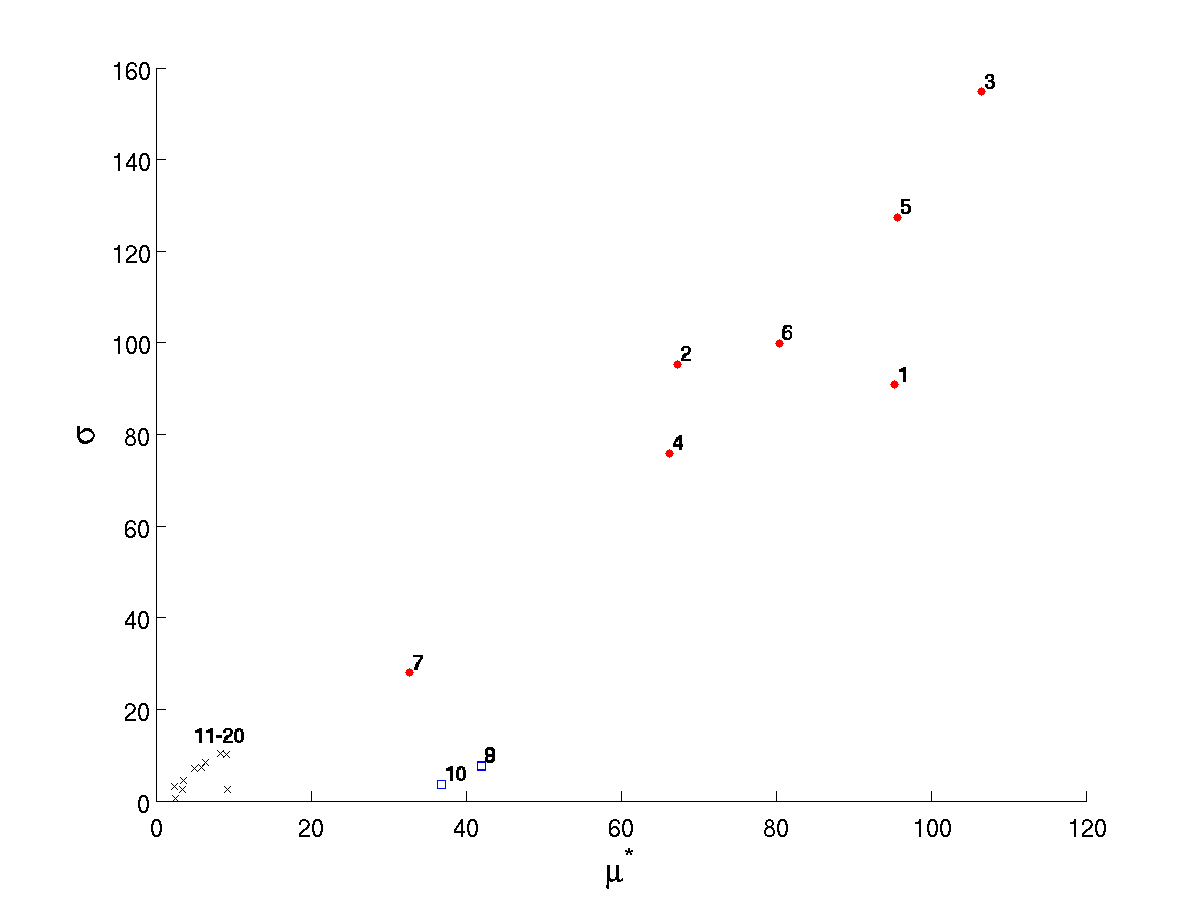
\includegraphics[width=\textwidth]{images/moat_mustar_sigma}
\caption{\label{FIG:mustar_sigma} Standard deviation of elementary
effects plotted against modified mean for Morris for each of 20
inputs. Red circles 1--7 correspond to inputs having interactions or
nonlinear effects, blue squares 8--10 indicate those with mainly
linear effects, and black Xs denote insignificant inputs.}
\end{figure}

